\documentclass[thesis]{subfiles}

\begin{document}

\OnlyInSubfile{\setcounter{chapter}{3}}
\chapter{First Principles simulations}
\label{sec:ab-initio}

As discussed in the previous chapter, to be able to compute the properties of a
system using statistical physics, we need to be able to compute the total energy
of this system in every possible configuration. It is possible to do so by
considering the quantum nature of the electrons, and solving the Schrödinger
equation for this system. We can still model the atomic nuclei as classical
particles, as this is usually sufficient for the description of the system.
Solving the Schrödinger equation to compute the energy of the system
presents the advantage that no additional hypotheses have to be made about the
system, and the functional form of the interaction potential $U(\r)$.

In this chapter, I will first introduce the Density Functional Theory (DFT)
approach used to solve the Schrödinger equation. I will then explain how I used
it to run \abinitio molecular dynamics to study deformations of \ZIF8 during
\ce{N2} adsorption. Finally, I will discuss how we can use DFT simulations to
parametrize classical force fields, allowing us to study bigger systems on
longer timescales at the cost of some accuracy.

\newpage
\section{From Schrödinger to Density Functional Theory}
\label{sec:dft}

\subsection{The Schrödinger equation}

In quantum chemistry, the state of a system is represented by a complex-valued
function of positions and time $\Psi(\r, t)$ called the \emph{wave function}.
The Schrödinger equation describes the time evolution of this wave function
given the Hamiltonian $\hat{\mathcal{H}}$ of the system\cite{Schrodinger1926}:
\[\hat{\mathcal{H}} \Psi(\r, t) = j\hbar \frac{\partial}{\partial t} \Psi(\r, t),\label{eq:time-schrodinger}\]
where $j$ is the imaginary number ($j^2 = -1$), and $\hbar$ the reduced Plank's
constant. The quantum Hamiltonian operator $\hat{\mathcal{H}}$ can be expressed
as a sum of quantum kinetic energy and potential energy operators:
\[\hat{\mathcal{H}} = \sum_i \frac{- \hbar^2}{2m_i} \nabla_i^2 + U(\r)\]
where the $m$ are the masses of the particles in the system, $\nabla$ is the
differential nabla operator, and $U(\r)$ is the potential energy of the system.
When the potential energy does not explicitly depend on time, we can look for
solution with separated variables of the form:
\[\Psi(\r, t) = \psi(\r) \times y(t).\]
Replacing in equation~\eqref{eq:time-schrodinger}, and separating the spatial
and time quantities, we get
\[- \sum \frac{\hbar^2}{2m} \frac{1}{\psi(\r)} \nabla^2 \psi(\r) + U(\r) = j\hbar \frac{1}{y(t)} \frac{\d y(t)}{\d t}.\]
For this equation to stand for all $t$ and all $r$, there must exist a constant
value $E$ such that:
\[j\hbar \frac{1}{y(t)} \frac{\d y(t)}{\d t} \quad = \quad E \quad = \quad - \sum \frac{\hbar^2}{2m} \frac{1}{\psi(\r)} \nabla^2 \psi(\r) + U(\r) \]

Putting everything together, any solution of the general
equation~\eqref{eq:time-schrodinger} can be written as a (potential infinite)
linear combination of special solutions:
\[\Psi(\r, t) = \sum_i^\infty c_i \ \psi_i(\r) \ e^{-j \ E_i \, t \, / \hbar},\]
with $c_i$ being the complex coefficients of the combination; and the $(E_i\ ;\
\psi_i)$ pairs are solutions of the \emph{time-independent} Schrödinger equation:
\[\hat{\mathcal{H}} \psi(\r) = E \psi(\r).\label{eq:schrodinger}\]
$\Psi$ is called a \emph{wave function} because its time dependence has a
wave-like form, and it propagates through space and time. Solving
equation~\eqref{eq:schrodinger} gives us stationary states $(E_i\ ;\ \psi_i)$,
where $E_i$ is the energy of the state; and $\psi_i$ is the wave function of the
state. Although there is no easy interpretation of the complex valued function
$\psi_i$, its squared norm $|\,\psi_i(\r)\,|^2$ is the probability density of
finding the electrons around a given position.

\subsection{Density Functional Theory}

To compute the energy of an atomic system, we need to solve
equation~\eqref{eq:schrodinger} for a collection of $N$ electrons carrying a
negative charge $-e$ and $M$ nuclei carrying a positive charge $e\,Z_j$, all
interacting through a Coulombic potential. As the electrons are much more
lightweight than the nuclei (an electron is roughly 2000 times lighter than a
proton), it is customary to work under the Born-Oppenheimer
approximation\cite{Born1927}. In this approximation, the degrees of freedom of
electrons and nuclei are decoupled, and the electrons move much faster than the
nuclei, reacting instantly to changes in the nuclei's positions. This
effectively means that at a given point in time, the electrons evolve in the
constant electrostatic potential generated by the fixed nuclei. The
corresponding Hamiltonian (using atomic units, \ie $e^2 / 4\pi\epsilon_0 = 1$;
$\hbar = 1$; and $m_\text{electron} = 1$) is:
\[\hat{\mathcal{H}} = \left[-\frac 1 2 \sum_i^N \nabla^2_i - \sum_i^N \sum_j^M \frac{Z_j}{|\r_i - \vec R_j|} + \sum_i^N \sum_{j>i}^N \frac{1}{|\r_i - \r_j|} \right].\]
We can rewrite this by defining the potential an electron feels due to the
presence of all the nuclei $V_\text{ext}(r) = -\sum_{j} Z_j / |\r - \vec R_j|$,
and the electron-electron interaction potential $U(r_i, r_j) = 1 / |\r_i -
\r_j|$:
\[\hat{\mathcal{H}} = \left[-\frac 12\sum_{i=1}^N \nabla^2_i + \sum_{i=1}^N V_\text{ext}(\r_i) + \sum_{i=1}^N \sum_{j>i}^N U(\r_i, \r_j)\right], \]
\[\hat{\mathcal{H}} = \hat T + \hat V_\text{ext} + \hat V_{ee}. \label{eq:electronic-hamiltonian}\]
The three terms in the Hamiltonian are the kinetic energy $\hat T$, the total
external potential $\hat V_\text{ext}$, and the electron-electron interaction
potential $\hat V_{ee}$. This electron-electron interaction makes the state of
any electron depend on the state of all other electrons; thus making the wave
function depends on $3N$ coupled variables. Looking directly for analytic or
numerical solutions of the Schrödinger equation is hard because the search space
is huge: even for small systems, they are already thousands of electrons
interacting.

The Density Functional Theory (DFT) is a strategy to solve the Schrödinger
equation without having to explicitly determine the wave function $\psi$. It is
based on the fact that the square of the norm of the wave function is the
probability for the system to be in a given state. For a system of electrons
evolving in the fixed potential created by the nuclei, the wave function
$\psi(\{\vec x\})$ depends on the Cartesian coordinates of all the electrons
$\{\vec x\}$. The electronic density $n(\r)$ is the probability to find an
electron in small neighboring of $\r$, defined as:
\[n(\r) = N \iiint |\psi(\r, \vec x_2, \cdots, \vec x_N)|^2 \ \d \vec x_2 \cdots\d \vec x_N \label{eq:electron-density}\]
The whole idea of DFT is to transform the problem so that we can look for
a solution of the Schrödinger equation as a function of 3 variables $n(\r)$
instead of a function of $3N$ variables $\psi$.

Hohenberg and Kohn showed in 1964\cite{Hohenberg1964} that every electronic
density correspond exactly to one and only one external potential
$V_\text{ext}$, \ie the knowledge of the external potential or the density are
equivalent. This is the first Hohenberg and Kohn theorem. This also means that
knowing the electronic density is equivalent to knowing the wave function of the
system, as one can reconstruct it using equation~\eqref{eq:schrodinger}. As a
consequence, all the observables of the system only depend on the electronic
density, and can be written as functionals of this density: $E[n]$, $\Psi[n]$,
\etc

The second Hohenberg and Kohn theorem\cite{Hohenberg1964} states that the ground
state electronic density $n_0(\r)$ is the one that minimize the energy
functional: $E[n] \geq E_0 = E[n_0]$. From the previous relations, the total
energy functional contains three terms:
\[E[n] = T[n] + V_\text{ext}[n] + V_{ee}[n];\]
where the potential terms can be expressed as integrals of the one and two
electrons density:
\[ V_\text{ext}[n] = \int V_\text{ext}(\r) \ n(\r) \ \d \r;\]
\[ V_{ee}[n] = \iint \frac{n_2(\r_1, \r_2)}{|\r_1 - \r_2|} \ \d \r_1 \d \r_2.\]
Here, the two electrons density $n_2(\r_1, \r_2)$ is the probability for an
electron to be in a small neighboring of $\r_1$, while another electron is in a
small neighboring of $\r_2$:
\[n_2(\r_1, \r_2) = N \iiint |\psi(\r_1, \r_2, \vec x_3, \cdots, \vec x_N)|^2 \ \d \vec x_3 \cdots\d \vec x_N.\]

While we can compute and minimize $V_\text{ext}[n]$ given the positions of the
nuclei, the two other terms $T[n]$ and $V_{ee}[n]$ are harder to evaluate.

Kohn and Sham reformulated the problem in 1965\cite{Kohn1965} by considering a
set of \emph{non-interacting} electrons evolving in a specific external
potential, such as the density arising from these electrons is the same as the
one we look for. The new system of non-interacting electrons is described by a
new set of independent orbitals $\phi_i$, such as the total electronic density
of the system is
\[n(\r) = \sum_i^N \left| \phi_i(\r) \right|^2.\]

For these non interacting electrons, the kinetic energy $T_s[n]$ is known:
\[T_s[n] = \sum_i^N \int \phi_i^*(\r) \left( -\frac 12 \nabla^2 \right) \phi_i(\r) \ \d\r.\]
We also know that most of the $V_{ee}[n]$ term can be approximated as a
classical classical Coulombic interaction --- the so called \emph{Hartree
energy} --- which we can compute directly from the electronic density:
\[V_H[n] = \iint \frac{n(\r_1) n(\r_2)}{|\r_1 - \r_2|} \ \d \r_1 \d \r_2.\]
The functional to minimize in order to find the electronic density is now
\[E[n] = T_s[n] + V_\text{ext}[n] + V_H[n] + E_{xc}[n],\label{eq:energy-functional}\]
in which we can compute all of the terms expect for the exchange-correlation
contribution $E_{xc}[n]$.
\[E_{xc}[n] = (T[n] - T_s[n]) + (V_{ee}[n] - V_H[n]).\]
The form of this contribution is generally unknown, and it describes the quantum
nature of electrons that are able to interact with themselves. The
"exchange-correlation" name comes from the two different physical terms that it
encompasses. The exchange energy is a quantum-only effect due to the fact that
electrons are not distinguishable, and that exchanging two of them should change
the sign of the wave function. This exchange effect is sometimes called Pauli
repulsion, as it increases the distance between the electrons. The correlation
term describes how much the presence of other electrons influences the position
of a given electron; \ie how much the two electrons density $n_2(\r_1, \r_2)$
differs from the product of single electrons densities $n(\r_1)n(\r_2)$.

It can be shown that the minimizing the energy functional is equivalent to
solving a set of differential equations called the Kohn-Sham equations:
\[ \left[-\frac 12 \nabla^2 + V_\text{ext}(\r) + \frac{\partial V_H[n](\r)}{\partial n(\vec r)} + \frac{\partial E_{xc}[n](\r)}{\partial n(\vec r)} \right] \phi_i = \epsilon_i \phi_i \label{eq:kohn-sham}\]
These are non-linear equations, as both $V_H[n]$ and $E_{xc}[n]$ depends on the
$\phi_i$ through $n(\r)$. The usual algorithm to solve them is a self-consistent
iterative algorithm. We start by making an initial guess for the Kohn-Sham
orbitals $\phi_i^0$, using for example a linear combination of atomic orbitals.
Using this initial guess, we can:
\begin{enumerate}
    \item calculate the corresponding electron density at step $\alpha$, $n^{\,\alpha}(\r)$;
    \item calculate all the terms in the left hand side of equation~\eqref{eq:kohn-sham}:
          kinetic, external, Hartree and exchange-correlation energies using this electron density;
    \item solve the Kohn-Sham equation to find new Kohn-Sham orbitals $\phi_i^{\,\alpha+1}$;
    \item compute the new energy using the energy functional~\eqref{eq:energy-functional}.
\end{enumerate}

If the new energy $E^{\,\alpha+1}$ and density $n^{\,\alpha+1}(\r)$ are the same
as the energy $E^{\,\alpha}$ and density $n^{\,\alpha}(\r)$ in the previous
step, then we have found the fixed point of the Kohn-Sham equation, and the
converged density is the solution of the Schrödinger equation. Else, we go back
to step 1 using the new Kohn-Sham orbitals as the initial guess. This cycle is
called the \emph{Self-Consistent Field} (SCF) method, as we iteratively solve
the equations until the solution is self-consistent.

When a solution is found, the ground state energy $E^{\,\alpha + 1}$ and
electronic density $n^{\,\alpha + 1}(\r)$ will be the values minimizing the
energy functional from equation~\eqref{eq:energy-functional}. The Kohn-Sham
energies $\{\,\epsilon_i\,\}$ on the other hand have no physical meaning. They
are only the solution of equation~\eqref{eq:kohn-sham} for a system of
non-interacting electrons that happens to have the same electronic density as
the real system of interest.

\subsection{Exchange, correlation, and dispersion}

A good approximation for the exchange-correlation functional is required to
solve the Kohn-Sham equations. There are a number of approaches routinely used
in theoretical chemistry, usually classified along the so-called Perdew's
ladder\cite{Perdew2001} from less precise and cheaper to compute to more precise
and expensive to compute. Going up the ladder, we encounter Local Density
Approximation (LDA) where the exchange-correlation functional only depends on
the local density; Generalized Gradient Approximation (GGA), where the
functional also depends on the local gradient of the density, meta-GGA
functionals incorporating the second derivative of the density (the Laplacian of
the density), or hybrid functionals. Hybrid functionals mix exchange expressions
from LDA or GGA with exact exchange term coming from other methods for solving
the Schrödinger equation, such as Hartree-Fock methods.

Generally, we use exchange-correlation functionals that only depend on the local
density, and maybe some of its derivatives. This means that DFT calculations
will have trouble reproducing non-electrostatic long-range correlation effects,
such as the dispersion interaction. Fortunately, we have a simple analytic
formulation for these interactions, which Grimme and coworkers\cite{Grimme2006,
Grimme2010} proposed to include when computing the total energy. This empirical
correction is added to the energy obtained by DFT, and does not directly modify
the electronic density.
\[E_\text{tot} = E_\text{DFT} + E_\text{disp} \]

In my PhD, I used the DFT-D3 version of this correction\cite{Grimme2010}, with
zero damping and only the two-body term. The correction to the energy is
expressed as:
\[E_\text{disp} = - \sum_i^M\sum_{j>i}^M\left[\frac{C_6^{ij}}{R_{ij}^{\,6}} \ f_6^{ij}(R_{ij}) + \frac{C_8^{ij}}{R_{ij}^{\,8}} \ f_8^{ij}(R_{ij})\right],\]
where the sum is over all the pairs of atoms, $R_{ij}$ is the distance between
the atoms, the $C_6^{ij}$ are parameters tabulated for each element pairs and
$f_n^{ij}$ is a damping function.
\[f_n^{ij}(R) =
\begin{dcases}
    \frac{s_n}{1 + 6 \left(R\ /\ \sigma_n \sqrt{C_8^{ij} / C_6^{ij}}\right)^{-\alpha_n}} &\text{for } R < R_c \\
    0 &\text{for } R \geq R_c \\
\end{dcases}\]
In this expression, $s_n$ and $\sigma_n$ are parameters specifically adapted to
the ex\-change-cor\-rela\-tion functional one uses. For example, when using the
PBE functional one should set $s_6 = 1.0$, $s_8 = 0.722$, $\sigma_6 = 1.217$,
and $\sigma_8 = 1.0$. $\alpha_6$ is always set to 14, and $\alpha_8$ to 16.

\subsection{Ab initio molecular dynamics}

DFT can be used to compute the energy and forces acting on the atoms during an
\abinitio molecular dynamics (AIMD) simulation. Different types of dynamics can
be used for the nuclei depending on the time precision needed, I only used the
Born-Oppenheimer dynamic. In this framework, the nuclei are supposed to behave
as classical particles, and DFT is used to optimize the electronic density at
each step of the dynamic. All the algorithms devised for molecular dynamics (see
section~\ref{sec:molecular-dynamics}) can be used. In particular, it is possible
to use AIMD to sample the $NVE$, $NVT$ and $NPT$ ensembles; although simulation
in the $NPT$ ensemble are more costly than simulations in the $NVT$ ensemble,
because the proper calculation of the pressure requires more precise atomic
forces, and a stricter convergence criterion in the SCF cycles.

\newpage
\section{Adsorption of \ce{N2} in \ZIF8 and its derivatives}
\label{sec:zif8x}

In this section, I will show an example of how the use of \abinitio molecular
dynamics enables a precise description of the adsorbed phase in flexible porous
materials. This study has been published in \citejournal{Chaplais2018}\cite{Chaplais2018}.

\subsection{\ZIF8 and its cousins}

The flexible porous material used in this study is \ZIF8. It is a representative
of the Zeolitic Imidazolate Framework (ZIF) family of MOFs, with a sodalite
(SOD) topology, methyl-imidazolate linkers, and zinc metallic centers. The
structure of \ZIF8 is represented in figure~\ref{fig:zif8-ch3:structure}.

\begin{figure}[ht]
    \centering
    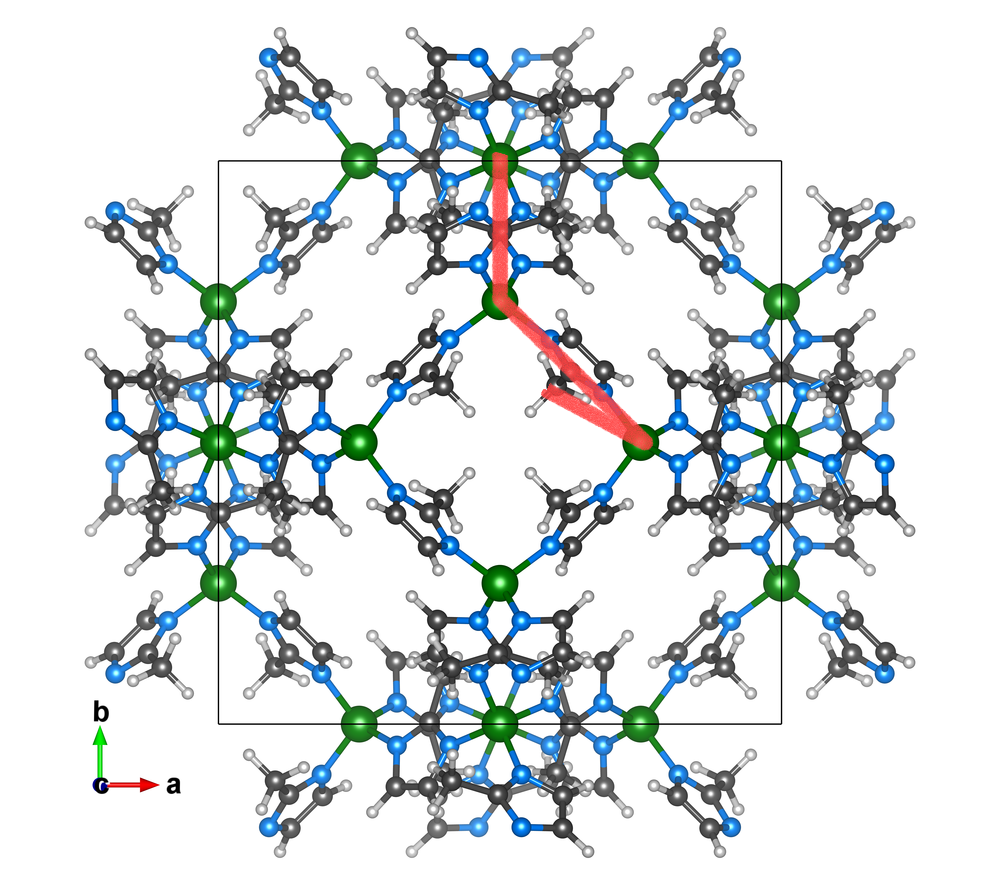
\includegraphics[width=0.45\textwidth]{figures/images/swing-angle}
    \hfill
    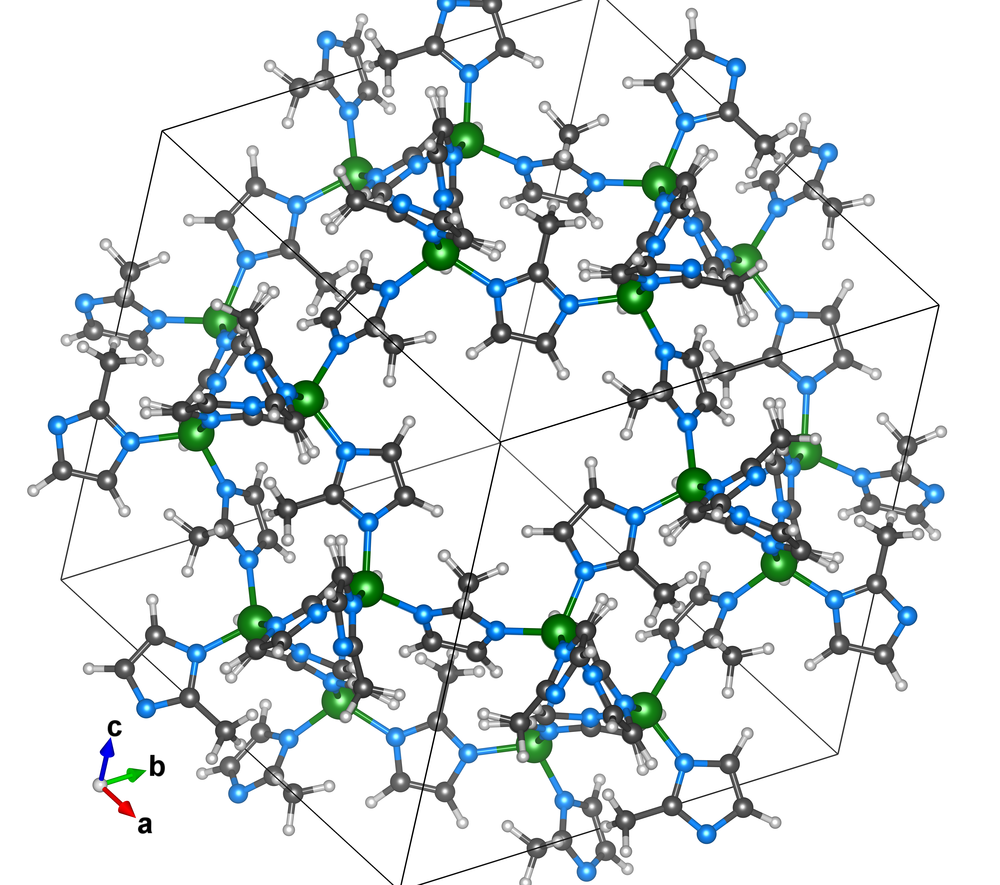
\includegraphics[width=0.45\textwidth]{figures/images/ZIF8-111}
    \caption{Structure of the methyl-imidazolate \ZIF8. On the left, the
    front-most opening is the 4-member ring window (the structure is represented
    along the 001 axis); and on the right the front-most opening is the 6-member
    ring window (the structure is represented along the 111 axis). The atomic
    color code is green for zinc, blue for nitrogen, gray for carbon and white
    for hydrogen. The red line connects the atoms of the "swing"
    \ce{Zn-Zn-Zn-X} dihedral angle.}
    \label{fig:zif8-ch3:structure}
\end{figure}

\ZIF8 is known for it relatively high surface area of \SI{1.947}{m^2/g} and
large cavity with a diameter of \SI{11.6}{\AA}\cite{Park2006}, separated by
6-ring windows of small diameter ($\approx$ \SI{3.4}{\AA}). It is also
commercially available and have excellent performance at the lab scale for the
separation of gas mixtures such as \ce{C2}/\ce{C3} hydrocarbons,
\ce{CO2}/\ce{CH4}, or \ce{CO2}/\ce{N2}\cite{Li2009, Bux2011}.

It exhibits some flexibility of its framework through torsional rotation of the
linkers around the plane defined by the 6-member ring windows. The first
evidence of such flexibility came from the fact that molecules bigger than the
window aperture can diffuse through the structure. When a molecule bigger than
the geometric window size tries to go through the window, the linkers will
rotate, effectively increasing the apparent window size. In particular, it has
been shown that we need to account for the flexibility of the structure to be
able to properly reproduce experimental diffusion coefficients of small
hydrocarbons\cite{Verploegh2015} when using molecular simulation.

Moreover, there is evidence of a structural transition occurring in \ZIF8 upon
loading, from an ambient pressure or AP phase to a high pressure or HP phase.
This was demonstrated using \emph{in situ} X-ray diffraction both during
methanol/ethanol intrusion at \SI{1,47}{GPa}\cite{Moggach2009}; and during the
adsorption of \ce{N2} at \SI{77}{K}\cite{FairenJimenez2011}. In the latter case,
the authors also demonstrated that the stepped isotherm (see
figure~\ref{fig:zif8x:isotherms}) could not be reproduced by Grand Canonical
Monte Carlo (GCMC) simulations in the rigid AP structure. Instead, they showed
that the lower pressure regime is reproduced by GCMC simulations in the rigid AP
structure, while the higher regime corresponds to GCMC simulations in the rigid
HP structure.

The AP and HP phases have the same space group ($I\bar{4}3m$), and mainly differ
by the orientation of the linkers around the 4 and 6-member windows. This
orientation is defined by the dihedral angle \ce{Zn-Zn-Zn-CH3}, also called the
\emph{swing angle}; which goes from an average value of 7° in the AP phase to an
average value of 35° in the HP phase.\cite{FairenJimenez2011} This angle is
represented in figure~\ref{fig:zif8-ch3:structure}. A recent, more detailed
characterization of the structural evolution upon adsorption showed that the
transition from AP to HP is a continuous rotation of the linkers, and not an
abrupt change.\cite{Coudert2017}.

Other studies\cite{FairenJimenez2012, Ania2012} showed that the adsorption
isotherms of \ce{CO}, \ce{O2} and \ce{Ar} at \SI{77}{K} and \SI{90}{K} all
present similar stepped isotherm and hysteresis loop in the high pressure
regime. Again, these isotherms could not be fully described by GCMC simulations
in the AP structure only, instead we also need to account for the HP phase.

\subsubsection{Nitrogen adsorption isotherms in \ZIF8, \ZIFCl, and \ZIFBr}

Two new materials analogs to \ZIF8 have been synthesized recently by
\citeauthor{Li2009}\cite{Li2009} using chloro- and bromo-substituted imidazolate
linkers instead of the original methyl-imidazolate in \ZIF8. These new
materials, that we will call \ZIFCl and \ZIFBr, are represented in
figure~\ref{fig:zif8x:structures}.

\begin{figure}[ht]
    \centering
    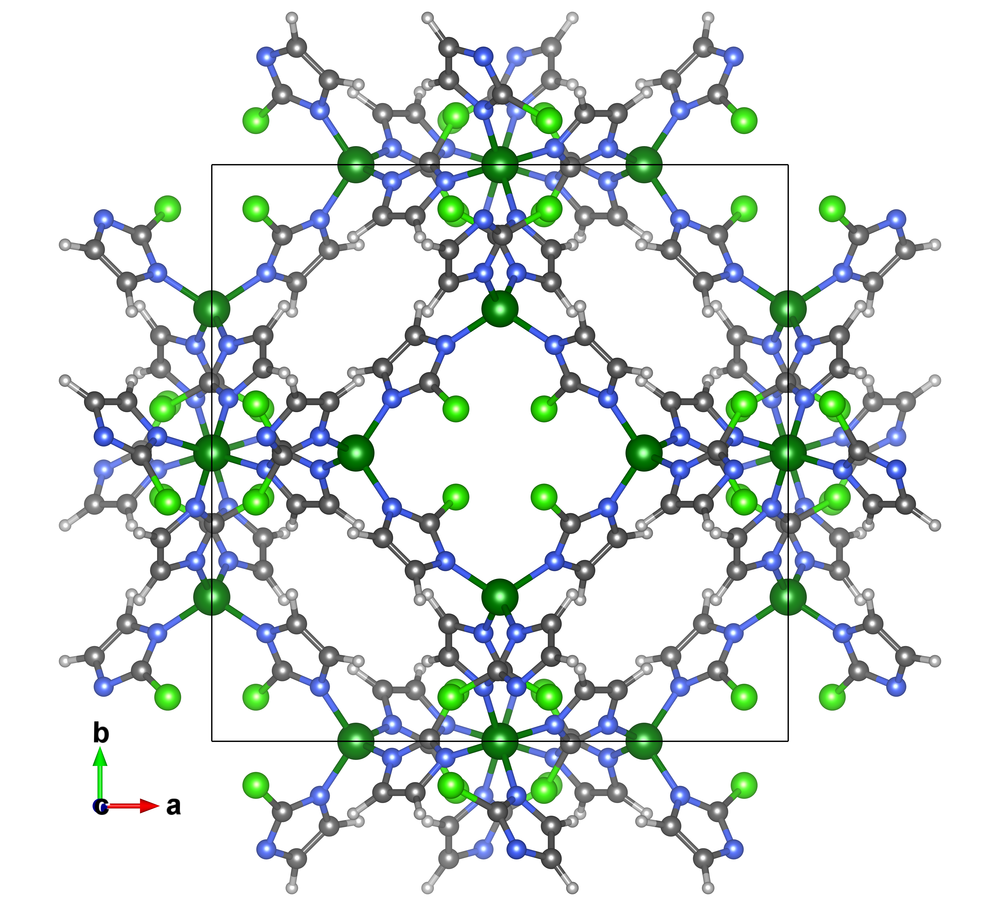
\includegraphics[width=0.45\textwidth]{figures/images/ZIF8-Cl}
    \hfill
    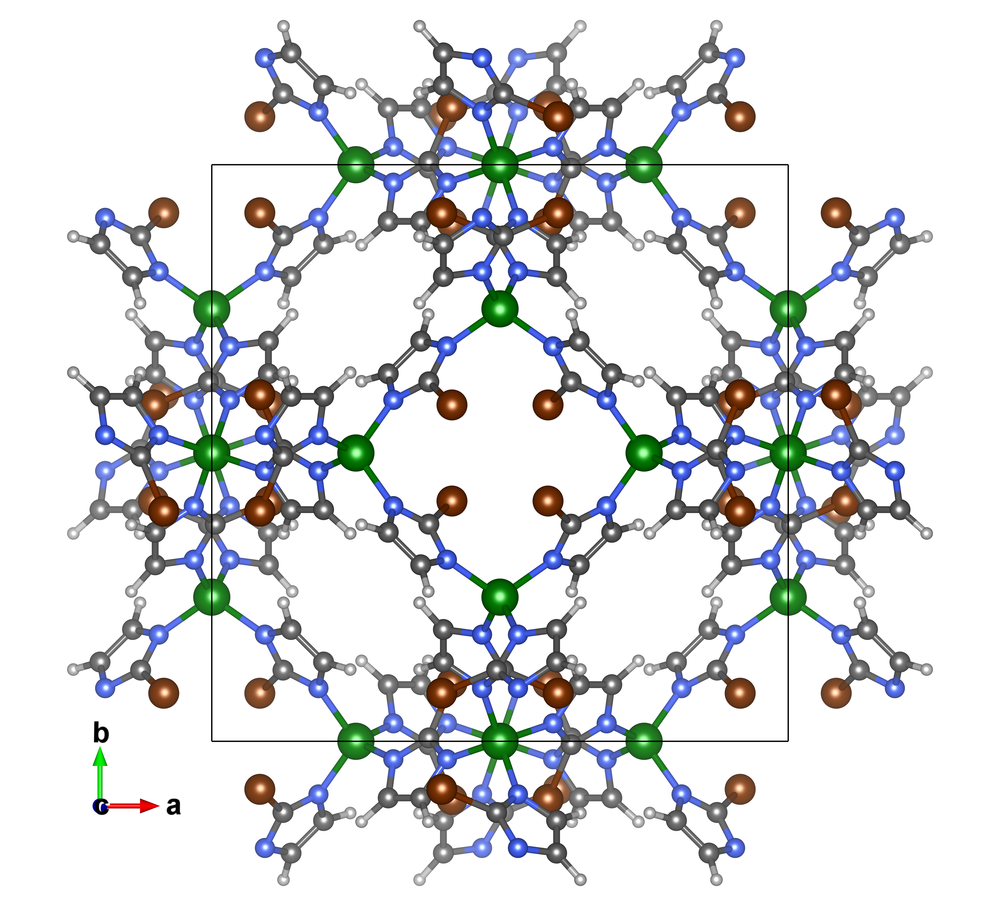
\includegraphics[width=0.45\textwidth]{figures/images/ZIF8-Br}
    \caption{Structure of the chloro-imidazolate \ZIFCl on the left and the
    bromo-imidazolate \ZIFBr on the right. The atomic color code is the same
    as in figure~\ref{fig:zif8-ch3:structure}, with a bright green for chlorine
    atoms and dark red for bromide atoms.}
    \label{fig:zif8x:structures}
\end{figure}

The nitrogen adsorption isotherms at \SI{77}{K} in \ZIF8, \ZIFCl and \ZIFBr, are
presented in figure~\ref{fig:zif8x:isotherms}. They were measured as part of a
collaboration by the experimental team IS2M laboratory in Université de
Haute Alsace, France.

\begin{figure}[ht]
    \centering
    % GNUPLOT: LaTeX picture with Postscript
\begingroup
  \makeatletter
  \providecommand\color[2][]{%
    \GenericError{(gnuplot) \space\space\space\@spaces}{%
      Package color not loaded in conjunction with
      terminal option `colourtext'%
    }{See the gnuplot documentation for explanation.%
    }{Either use 'blacktext' in gnuplot or load the package
      color.sty in LaTeX.}%
    \renewcommand\color[2][]{}%
  }%
  \providecommand\includegraphics[2][]{%
    \GenericError{(gnuplot) \space\space\space\@spaces}{%
      Package graphicx or graphics not loaded%
    }{See the gnuplot documentation for explanation.%
    }{The gnuplot epslatex terminal needs graphicx.sty or graphics.sty.}%
    \renewcommand\includegraphics[2][]{}%
  }%
  \providecommand\rotatebox[2]{#2}%
  \@ifundefined{ifGPcolor}{%
    \newif\ifGPcolor
    \GPcolortrue
  }{}%
  \@ifundefined{ifGPblacktext}{%
    \newif\ifGPblacktext
    \GPblacktextfalse
  }{}%
  % define a \g@addto@macro without @ in the name:
  \let\gplgaddtomacro\g@addto@macro
  % define empty templates for all commands taking text:
  \gdef\gplbacktext{}%
  \gdef\gplfronttext{}%
  \makeatother
  \ifGPblacktext
    % no textcolor at all
    \def\colorrgb#1{}%
    \def\colorgray#1{}%
  \else
    % gray or color?
    \ifGPcolor
      \def\colorrgb#1{\color[rgb]{#1}}%
      \def\colorgray#1{\color[gray]{#1}}%
      \expandafter\def\csname LTw\endcsname{\color{white}}%
      \expandafter\def\csname LTb\endcsname{\color{black}}%
      \expandafter\def\csname LTa\endcsname{\color{black}}%
      \expandafter\def\csname LT0\endcsname{\color[rgb]{1,0,0}}%
      \expandafter\def\csname LT1\endcsname{\color[rgb]{0,1,0}}%
      \expandafter\def\csname LT2\endcsname{\color[rgb]{0,0,1}}%
      \expandafter\def\csname LT3\endcsname{\color[rgb]{1,0,1}}%
      \expandafter\def\csname LT4\endcsname{\color[rgb]{0,1,1}}%
      \expandafter\def\csname LT5\endcsname{\color[rgb]{1,1,0}}%
      \expandafter\def\csname LT6\endcsname{\color[rgb]{0,0,0}}%
      \expandafter\def\csname LT7\endcsname{\color[rgb]{1,0.3,0}}%
      \expandafter\def\csname LT8\endcsname{\color[rgb]{0.5,0.5,0.5}}%
    \else
      % gray
      \def\colorrgb#1{\color{black}}%
      \def\colorgray#1{\color[gray]{#1}}%
      \expandafter\def\csname LTw\endcsname{\color{white}}%
      \expandafter\def\csname LTb\endcsname{\color{black}}%
      \expandafter\def\csname LTa\endcsname{\color{black}}%
      \expandafter\def\csname LT0\endcsname{\color{black}}%
      \expandafter\def\csname LT1\endcsname{\color{black}}%
      \expandafter\def\csname LT2\endcsname{\color{black}}%
      \expandafter\def\csname LT3\endcsname{\color{black}}%
      \expandafter\def\csname LT4\endcsname{\color{black}}%
      \expandafter\def\csname LT5\endcsname{\color{black}}%
      \expandafter\def\csname LT6\endcsname{\color{black}}%
      \expandafter\def\csname LT7\endcsname{\color{black}}%
      \expandafter\def\csname LT8\endcsname{\color{black}}%
    \fi
  \fi
    \setlength{\unitlength}{0.0500bp}%
    \ifx\gptboxheight\undefined%
      \newlength{\gptboxheight}%
      \newlength{\gptboxwidth}%
      \newsavebox{\gptboxtext}%
    \fi%
    \setlength{\fboxrule}{0.5pt}%
    \setlength{\fboxsep}{1pt}%
\begin{picture}(5660.00,4240.00)%
    \gplgaddtomacro\gplbacktext{%
      \csname LTb\endcsname%%
      \put(752,694){\makebox(0,0)[r]{\strut{}$0$}}%
      \csname LTb\endcsname%%
      \put(752,1434){\makebox(0,0)[r]{\strut{}$100$}}%
      \csname LTb\endcsname%%
      \put(752,2173){\makebox(0,0)[r]{\strut{}$200$}}%
      \csname LTb\endcsname%%
      \put(752,2913){\makebox(0,0)[r]{\strut{}$300$}}%
      \csname LTb\endcsname%%
      \put(752,3652){\makebox(0,0)[r]{\strut{}$400$}}%
      \csname LTb\endcsname%%
      \put(1533,477){\makebox(0,0){\strut{}$10^{-4}$}}%
      \csname LTb\endcsname%%
      \put(2486,477){\makebox(0,0){\strut{}$10^{-3}$}}%
      \csname LTb\endcsname%%
      \put(3439,477){\makebox(0,0){\strut{}$10^{-2}$}}%
      \csname LTb\endcsname%%
      \put(4392,477){\makebox(0,0){\strut{}$10^{-1}$}}%
    }%
    \gplgaddtomacro\gplfronttext{%
      \csname LTb\endcsname%%
      \put(178,2358){\rotatebox{-270}{\makebox(0,0){\strut{}uptake (\si{cm^3/cm^3} STP)}}}%
      \csname LTb\endcsname%%
      \put(3086,152){\makebox(0,0){\strut{}$P / P_0$}}%
      \csname LTb\endcsname%%
      \put(4518,2249){\makebox(0,0)[r]{\strut{}\footnotesize\ZIFCH3}}%
      \csname LTb\endcsname%%
      \put(4518,2032){\makebox(0,0)[r]{\strut{}\footnotesize\ZIFCl}}%
      \csname LTb\endcsname%%
      \put(4518,1815){\makebox(0,0)[r]{\strut{}\footnotesize\ZIFBr}}%
    }%
    \gplbacktext
    \put(0,0){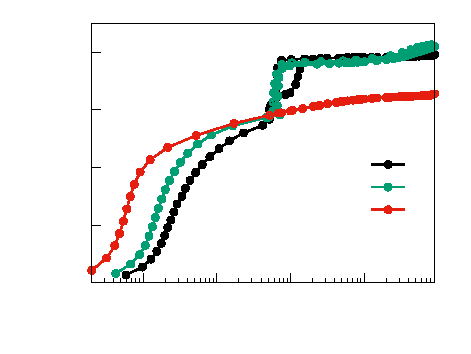
\includegraphics{zif8x-isotherms}}%
    \gplfronttext
  \end{picture}%
\endgroup

    \caption{Nitrogen adsorption isotherms at \SI{77}{K} in \ZIF8 (black) and
    the chloro (green) and bromo (red) derivatives. Full circles are used for
    the adsorption branch, and empty ones for the desorption branch.
    Experimental data acquired by \citeauthor{Chaplais2018}\cite{Chaplais2018}}
    \label{fig:zif8x:isotherms}
\end{figure}

Looking at these isotherms, we first notice that for \ZIF8, there are two jumps
in loading: a first one corresponding to the initial filling of the pores up
until around \SI{300}{cm^3/cm^3}, and a second one up until
\SI{400}{cm^3/cm^3}. This shape of isotherm is known as a type IV isotherm in
the International Union of Pure and Applied Chemistry (IUPAC)
classification\cite{Sing1985} (see figure~\ref{fig:iupac-isotherms}). Type IV
isotherms usually appear when two kinds of porosity exist, and the second, larger
kind is filled at higher pressures; for example when there are both micropores
and mesoscopic pores in the material. In the case of \ZIF8, there is no evidence
for the existence of such mesoscopic pores, and instead the step in the isotherm
is attributed to the phase transition between the AP and HP phases.

Concerning the two new materials, \ZIFCl shows the same behavior with a stepped,
type IV adsorption isotherm. \ZIFBr however presents a different isotherm shape,
without the second jump in loading, known as a type I isotherm in the IUPAC
classification. This kind of isotherm usually occurs in materials where there is
a single kind of micropores.

\subsubsection{\emph{Ab initio} molecular dynamics study}
\label{sec:zif8x:methods}

In order to gain better understanding of the relation between the structure
changes and the adsorbed molecules, I used molecular dynamics simulations. To
describe fully the flexibility of the frameworks without any assumption, I
favored \abinitio molecular dynamics over force field-based molecular dynamics
--- as there are currently no force fields available for the \ZIF8 variants
studied here, and existing force fields for \ZIFCH3 have questionable accuracy.
For each framework --- \ZIFCH3, \ZIFCl, \ZIFBr --- I ran five simulations
corresponding to different numbers of nitrogen molecules $N$ inside the porous
space, going from an empty framework ($N = 0$) to the fully loaded host
material. The maximal loading was determined from the experimental isotherms to
be close to $N = 50$ molecules per unit cell for \ZIFCH3 and \ZIFCl and $N = 40$
molecules per unit cell for \ZIFBr.

To create the starting configurations, I started from the energy-minimized
configuration of the empty frameworks, and randomly placed the selected number
of nitrogen molecules in the unit cell using the packmol
software\cite{Martnez2009}. The whole \{ZIF, adsorbate\} system was then
minimized again at the DFT level before starting the molecular dynamics
simulations. I used the Quickstep module\cite{VandeVondele2005} of the CP2K
software package (version 2.5.1, available online at http://www.cp2k.org/) for
all the simulations. I used a PBE exchange-correlation functional with D3
dispersion corrections, a double zeta polarizable valence (DZVP) basis set, and
an energetic cutoff of 600 Ry. All the systems were simulated with a \SI{1}{fs}
timestep giving a total of 12 to \SI{22}{ps} of simulation. Temperature was held
constant at 77 K with a CSVR thermostat, using a thermostat time constant of
\SI{1000}{fs}. I used the last \SI{5}{ps} of simulation for analysis, leaving 7
to \SI{17}{ps} to the system to reach equilibrium.

We used constant volume ($NVT$) simulations instead of constant pressure ($NPT$)
simulations because $NPT$ molecular dynamics simulations require a higher
computation time to correctly converge the calculation of forces. In general,
when global deformations are expected in the system, one should use $NPT$
simulation. In this case, I was able to use $NVT$ simulations because the volume
change between the different phases of \ZIFCH3 is very small. The low-pressure
phase unit cell volume is \SI{4900.5}{\AA^3}, while the high-pressure phase
volume is \SI{4974.8}{\AA^3}, making the difference less than 2\%.

\subsection{Deformation under adsorption}
\label{sec:zif8x:swing}

The first indicator of deformation of the framework is the \ce{Zn-Zn-Zn-X}
dihedral angle, where \ce{X} is the group on the imidazolate linkers: methyl,
chlorine or bromide. This angle --- presented on
figure~\ref{fig:zif8-ch3:structure} --- is also called the swing angle, noted
$\phi$. The swing angle represents the rotation of the linker around the 6-member
window plane, with 0° being the point where the linker is completely in this
plane.

\begin{figure}[ht]
    \centering
    % GNUPLOT: LaTeX picture with Postscript
\begingroup
  \makeatletter
  \providecommand\color[2][]{%
    \GenericError{(gnuplot) \space\space\space\@spaces}{%
      Package color not loaded in conjunction with
      terminal option `colourtext'%
    }{See the gnuplot documentation for explanation.%
    }{Either use 'blacktext' in gnuplot or load the package
      color.sty in LaTeX.}%
    \renewcommand\color[2][]{}%
  }%
  \providecommand\includegraphics[2][]{%
    \GenericError{(gnuplot) \space\space\space\@spaces}{%
      Package graphicx or graphics not loaded%
    }{See the gnuplot documentation for explanation.%
    }{The gnuplot epslatex terminal needs graphicx.sty or graphics.sty.}%
    \renewcommand\includegraphics[2][]{}%
  }%
  \providecommand\rotatebox[2]{#2}%
  \@ifundefined{ifGPcolor}{%
    \newif\ifGPcolor
    \GPcolortrue
  }{}%
  \@ifundefined{ifGPblacktext}{%
    \newif\ifGPblacktext
    \GPblacktextfalse
  }{}%
  % define a \g@addto@macro without @ in the name:
  \let\gplgaddtomacro\g@addto@macro
  % define empty templates for all commands taking text:
  \gdef\gplbacktext{}%
  \gdef\gplfronttext{}%
  \makeatother
  \ifGPblacktext
    % no textcolor at all
    \def\colorrgb#1{}%
    \def\colorgray#1{}%
  \else
    % gray or color?
    \ifGPcolor
      \def\colorrgb#1{\color[rgb]{#1}}%
      \def\colorgray#1{\color[gray]{#1}}%
      \expandafter\def\csname LTw\endcsname{\color{white}}%
      \expandafter\def\csname LTb\endcsname{\color{black}}%
      \expandafter\def\csname LTa\endcsname{\color{black}}%
      \expandafter\def\csname LT0\endcsname{\color[rgb]{1,0,0}}%
      \expandafter\def\csname LT1\endcsname{\color[rgb]{0,1,0}}%
      \expandafter\def\csname LT2\endcsname{\color[rgb]{0,0,1}}%
      \expandafter\def\csname LT3\endcsname{\color[rgb]{1,0,1}}%
      \expandafter\def\csname LT4\endcsname{\color[rgb]{0,1,1}}%
      \expandafter\def\csname LT5\endcsname{\color[rgb]{1,1,0}}%
      \expandafter\def\csname LT6\endcsname{\color[rgb]{0,0,0}}%
      \expandafter\def\csname LT7\endcsname{\color[rgb]{1,0.3,0}}%
      \expandafter\def\csname LT8\endcsname{\color[rgb]{0.5,0.5,0.5}}%
    \else
      % gray
      \def\colorrgb#1{\color{black}}%
      \def\colorgray#1{\color[gray]{#1}}%
      \expandafter\def\csname LTw\endcsname{\color{white}}%
      \expandafter\def\csname LTb\endcsname{\color{black}}%
      \expandafter\def\csname LTa\endcsname{\color{black}}%
      \expandafter\def\csname LT0\endcsname{\color{black}}%
      \expandafter\def\csname LT1\endcsname{\color{black}}%
      \expandafter\def\csname LT2\endcsname{\color{black}}%
      \expandafter\def\csname LT3\endcsname{\color{black}}%
      \expandafter\def\csname LT4\endcsname{\color{black}}%
      \expandafter\def\csname LT5\endcsname{\color{black}}%
      \expandafter\def\csname LT6\endcsname{\color{black}}%
      \expandafter\def\csname LT7\endcsname{\color{black}}%
      \expandafter\def\csname LT8\endcsname{\color{black}}%
    \fi
  \fi
    \setlength{\unitlength}{0.0500bp}%
    \ifx\gptboxheight\undefined%
      \newlength{\gptboxheight}%
      \newlength{\gptboxwidth}%
      \newsavebox{\gptboxtext}%
    \fi%
    \setlength{\fboxrule}{0.5pt}%
    \setlength{\fboxsep}{1pt}%
\begin{picture}(7760.00,3100.00)%
    \gplgaddtomacro\gplbacktext{%
      \csname LTb\endcsname%%
      \put(212,341){\makebox(0,0){\strut{}$0$}}%
      \csname LTb\endcsname%%
      \put(636,341){\makebox(0,0){\strut{}$10$}}%
      \csname LTb\endcsname%%
      \put(1060,341){\makebox(0,0){\strut{}$20$}}%
      \csname LTb\endcsname%%
      \put(1483,341){\makebox(0,0){\strut{}$30$}}%
      \csname LTb\endcsname%%
      \put(1907,341){\makebox(0,0){\strut{}$40$}}%
      \csname LTb\endcsname%%
      \put(2331,341){\makebox(0,0){\strut{}$50$}}%
    }%
    \gplgaddtomacro\gplfronttext{%
      \csname LTb\endcsname%%
      \put(1271,109){\makebox(0,0){\strut{}$\phi$ (°)}}%
      \csname LTb\endcsname%%
      \put(1271,2867){\makebox(0,0){\strut{}\ZIFCH3}}%
      \csname LTb\endcsname%%
      \put(1759,2494){\makebox(0,0)[r]{\strut{}\scriptsize 0 \ce{N2}}}%
      \csname LTb\endcsname%%
      \put(1759,2339){\makebox(0,0)[r]{\strut{}\scriptsize 10 \ce{N2}}}%
      \csname LTb\endcsname%%
      \put(1759,2184){\makebox(0,0)[r]{\strut{}\scriptsize 25 \ce{N2}}}%
      \csname LTb\endcsname%%
      \put(1759,2029){\makebox(0,0)[r]{\strut{}\scriptsize 40 \ce{N2}}}%
      \csname LTb\endcsname%%
      \put(1759,1874){\makebox(0,0)[r]{\strut{}\scriptsize 50 \ce{N2}}}%
    }%
    \gplgaddtomacro\gplbacktext{%
      \csname LTb\endcsname%%
      \put(2628,341){\makebox(0,0){\strut{}$0$}}%
      \csname LTb\endcsname%%
      \put(3086,341){\makebox(0,0){\strut{}$10$}}%
      \csname LTb\endcsname%%
      \put(3544,341){\makebox(0,0){\strut{}$20$}}%
      \csname LTb\endcsname%%
      \put(4001,341){\makebox(0,0){\strut{}$30$}}%
      \csname LTb\endcsname%%
      \put(4459,341){\makebox(0,0){\strut{}$40$}}%
      \csname LTb\endcsname%%
      \put(4917,341){\makebox(0,0){\strut{}$50$}}%
    }%
    \gplgaddtomacro\gplfronttext{%
      \csname LTb\endcsname%%
      \put(3772,109){\makebox(0,0){\strut{}$\phi$ (°)}}%
      \csname LTb\endcsname%%
      \put(3772,2867){\makebox(0,0){\strut{}\ZIFCl}}%
      \csname LTb\endcsname%%
      \put(4345,2494){\makebox(0,0)[r]{\strut{}\scriptsize 0 \ce{N2}}}%
      \csname LTb\endcsname%%
      \put(4345,2339){\makebox(0,0)[r]{\strut{}\scriptsize 10 \ce{N2}}}%
      \csname LTb\endcsname%%
      \put(4345,2184){\makebox(0,0)[r]{\strut{}\scriptsize 25 \ce{N2}}}%
      \csname LTb\endcsname%%
      \put(4345,2029){\makebox(0,0)[r]{\strut{}\scriptsize 40 \ce{N2}}}%
      \csname LTb\endcsname%%
      \put(4345,1874){\makebox(0,0)[r]{\strut{}\scriptsize 50 \ce{N2}}}%
    }%
    \gplgaddtomacro\gplbacktext{%
      \csname LTb\endcsname%%
      \put(5215,341){\makebox(0,0){\strut{}$0$}}%
      \csname LTb\endcsname%%
      \put(5673,341){\makebox(0,0){\strut{}$10$}}%
      \csname LTb\endcsname%%
      \put(6131,341){\makebox(0,0){\strut{}$20$}}%
      \csname LTb\endcsname%%
      \put(6588,341){\makebox(0,0){\strut{}$30$}}%
      \csname LTb\endcsname%%
      \put(7046,341){\makebox(0,0){\strut{}$40$}}%
      \csname LTb\endcsname%%
      \put(7504,341){\makebox(0,0){\strut{}$50$}}%
    }%
    \gplgaddtomacro\gplfronttext{%
      \csname LTb\endcsname%%
      \put(6359,109){\makebox(0,0){\strut{}$\phi$ (°)}}%
      \csname LTb\endcsname%%
      \put(6359,2867){\makebox(0,0){\strut{}\ZIFBr}}%
      \csname LTb\endcsname%%
      \put(6932,2494){\makebox(0,0)[r]{\strut{}\scriptsize 0 \ce{N2}}}%
      \csname LTb\endcsname%%
      \put(6932,2339){\makebox(0,0)[r]{\strut{}\scriptsize 8 \ce{N2}}}%
      \csname LTb\endcsname%%
      \put(6932,2184){\makebox(0,0)[r]{\strut{}\scriptsize 20 \ce{N2}}}%
      \csname LTb\endcsname%%
      \put(6932,2029){\makebox(0,0)[r]{\strut{}\scriptsize 40 \ce{N2}}}%
      \csname LTb\endcsname%%
      \put(6932,1874){\makebox(0,0)[r]{\strut{}\scriptsize 50 \ce{N2}}}%
    }%
    \gplbacktext
    \put(0,0){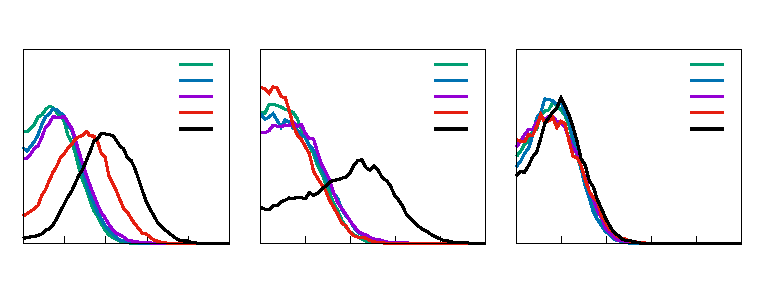
\includegraphics{zif8x-dihedrals}}%
    \gplfronttext
  \end{picture}%
\endgroup

    \caption{Distribution of linker swing angle (\ce{Zn-Zn-Zn-X} dihedral angle,
    where \ce{X} stands for \ce{CH3}, \ce{Cl} or \ce{Br} for \ZIFCH3, \ZIFCl or
    \ZIFBr, respectively) at various values of nitrogen loading.}
    \label{fig:zif8x:dihedrals}
\end{figure}

Following the evolution of the distribution of swing angles as the number of
nitrogen molecules increases allow understanding the deformations of the three
frameworks under adsorption. This evolution is represented on
figure~\ref{fig:zif8x:dihedrals}, where we observe a gradual increase of the
mean angle value as loading increases while the distribution remains
Gaussian-like.

These results are consistent with the already published ones for
\ZIFCH3\cite{Coudert2017}, but using a different functional (PBE here instead of
BLYP in reference~\cite{Coudert2017}). Interestingly, the two other frameworks behave
differently. For \ZIFCl, almost no change is noticed in the distribution profile
upon adsorption until the highest value of loading (\ie, $N = 50$). In this
case, the distribution shifts and the profile is no longer of Gaussian type, but
instead looks like the sum of two Gaussian distribution, one centered around
25°, and the other one around 10°. This indicates that some of the linkers do not
rotate (swing) even at high loading. The non-zero value of the distribution at
$\phi = 0\text{°}$ contrasts with the case of \ZIFCH3. Finally, for \ZIFBr, no
significant change occurs for the dihedral angle distribution as the loading
increases, meaning that the linkers do not rotate.

\begin{figure}[t]
    \centering
    % GNUPLOT: LaTeX picture with Postscript
\begingroup
  \makeatletter
  \providecommand\color[2][]{%
    \GenericError{(gnuplot) \space\space\space\@spaces}{%
      Package color not loaded in conjunction with
      terminal option `colourtext'%
    }{See the gnuplot documentation for explanation.%
    }{Either use 'blacktext' in gnuplot or load the package
      color.sty in LaTeX.}%
    \renewcommand\color[2][]{}%
  }%
  \providecommand\includegraphics[2][]{%
    \GenericError{(gnuplot) \space\space\space\@spaces}{%
      Package graphicx or graphics not loaded%
    }{See the gnuplot documentation for explanation.%
    }{The gnuplot epslatex terminal needs graphicx.sty or graphics.sty.}%
    \renewcommand\includegraphics[2][]{}%
  }%
  \providecommand\rotatebox[2]{#2}%
  \@ifundefined{ifGPcolor}{%
    \newif\ifGPcolor
    \GPcolortrue
  }{}%
  \@ifundefined{ifGPblacktext}{%
    \newif\ifGPblacktext
    \GPblacktextfalse
  }{}%
  % define a \g@addto@macro without @ in the name:
  \let\gplgaddtomacro\g@addto@macro
  % define empty templates for all commands taking text:
  \gdef\gplbacktext{}%
  \gdef\gplfronttext{}%
  \makeatother
  \ifGPblacktext
    % no textcolor at all
    \def\colorrgb#1{}%
    \def\colorgray#1{}%
  \else
    % gray or color?
    \ifGPcolor
      \def\colorrgb#1{\color[rgb]{#1}}%
      \def\colorgray#1{\color[gray]{#1}}%
      \expandafter\def\csname LTw\endcsname{\color{white}}%
      \expandafter\def\csname LTb\endcsname{\color{black}}%
      \expandafter\def\csname LTa\endcsname{\color{black}}%
      \expandafter\def\csname LT0\endcsname{\color[rgb]{1,0,0}}%
      \expandafter\def\csname LT1\endcsname{\color[rgb]{0,1,0}}%
      \expandafter\def\csname LT2\endcsname{\color[rgb]{0,0,1}}%
      \expandafter\def\csname LT3\endcsname{\color[rgb]{1,0,1}}%
      \expandafter\def\csname LT4\endcsname{\color[rgb]{0,1,1}}%
      \expandafter\def\csname LT5\endcsname{\color[rgb]{1,1,0}}%
      \expandafter\def\csname LT6\endcsname{\color[rgb]{0,0,0}}%
      \expandafter\def\csname LT7\endcsname{\color[rgb]{1,0.3,0}}%
      \expandafter\def\csname LT8\endcsname{\color[rgb]{0.5,0.5,0.5}}%
    \else
      % gray
      \def\colorrgb#1{\color{black}}%
      \def\colorgray#1{\color[gray]{#1}}%
      \expandafter\def\csname LTw\endcsname{\color{white}}%
      \expandafter\def\csname LTb\endcsname{\color{black}}%
      \expandafter\def\csname LTa\endcsname{\color{black}}%
      \expandafter\def\csname LT0\endcsname{\color{black}}%
      \expandafter\def\csname LT1\endcsname{\color{black}}%
      \expandafter\def\csname LT2\endcsname{\color{black}}%
      \expandafter\def\csname LT3\endcsname{\color{black}}%
      \expandafter\def\csname LT4\endcsname{\color{black}}%
      \expandafter\def\csname LT5\endcsname{\color{black}}%
      \expandafter\def\csname LT6\endcsname{\color{black}}%
      \expandafter\def\csname LT7\endcsname{\color{black}}%
      \expandafter\def\csname LT8\endcsname{\color{black}}%
    \fi
  \fi
    \setlength{\unitlength}{0.0500bp}%
    \ifx\gptboxheight\undefined%
      \newlength{\gptboxheight}%
      \newlength{\gptboxwidth}%
      \newsavebox{\gptboxtext}%
    \fi%
    \setlength{\fboxrule}{0.5pt}%
    \setlength{\fboxsep}{1pt}%
\begin{picture}(7360.00,2820.00)%
    \gplgaddtomacro\gplbacktext{%
      \csname LTb\endcsname%%
      \put(274,341){\makebox(0,0){\strut{}$8$}}%
      \csname LTb\endcsname%%
      \put(755,341){\makebox(0,0){\strut{}$9$}}%
      \csname LTb\endcsname%%
      \put(1236,341){\makebox(0,0){\strut{}$10$}}%
      \csname LTb\endcsname%%
      \put(1717,341){\makebox(0,0){\strut{}$11$}}%
      \csname LTb\endcsname%%
      \put(2198,341){\makebox(0,0){\strut{}$12$}}%
    }%
    \gplgaddtomacro\gplfronttext{%
      \csname LTb\endcsname%%
      \put(42,1425){\rotatebox{-270}{\makebox(0,0){\strut{}\scriptsize pore size distribution (log scale)}}}%
      \csname LTb\endcsname%%
      \put(1236,109){\makebox(0,0){\strut{}\scriptsize pore size (\AA)}}%
      \csname LTb\endcsname%%
      \put(1236,2587){\makebox(0,0){\strut{}\ZIFCH3}}%
      \csname LTb\endcsname%%
      \put(727,2183){\makebox(0,0)[r]{\strut{}\scriptsize 0 \ce{N2}}}%
      \csname LTb\endcsname%%
      \put(727,2028){\makebox(0,0)[r]{\strut{}\scriptsize 10 \ce{N2}}}%
      \csname LTb\endcsname%%
      \put(727,1873){\makebox(0,0)[r]{\strut{}\scriptsize 25 \ce{N2}}}%
      \csname LTb\endcsname%%
      \put(727,1718){\makebox(0,0)[r]{\strut{}\scriptsize 40 \ce{N2}}}%
      \csname LTb\endcsname%%
      \put(727,1563){\makebox(0,0)[r]{\strut{}\scriptsize 50 \ce{N2}}}%
    }%
    \gplgaddtomacro\gplbacktext{%
      \csname LTb\endcsname%%
      \put(2495,341){\makebox(0,0){\strut{}$8$}}%
      \csname LTb\endcsname%%
      \put(3034,341){\makebox(0,0){\strut{}$9$}}%
      \csname LTb\endcsname%%
      \put(3573,341){\makebox(0,0){\strut{}$10$}}%
      \csname LTb\endcsname%%
      \put(4112,341){\makebox(0,0){\strut{}$11$}}%
      \csname LTb\endcsname%%
      \put(4651,341){\makebox(0,0){\strut{}$12$}}%
    }%
    \gplgaddtomacro\gplfronttext{%
      \csname LTb\endcsname%%
      \put(3573,109){\makebox(0,0){\strut{}\scriptsize pore size (\AA)}}%
      \csname LTb\endcsname%%
      \put(3573,2587){\makebox(0,0){\strut{}\ZIFCl}}%
      \csname LTb\endcsname%%
      \put(3040,2183){\makebox(0,0)[r]{\strut{}\scriptsize 0 \ce{N2}}}%
      \csname LTb\endcsname%%
      \put(3040,2028){\makebox(0,0)[r]{\strut{}\scriptsize 10 \ce{N2}}}%
      \csname LTb\endcsname%%
      \put(3040,1873){\makebox(0,0)[r]{\strut{}\scriptsize 25 \ce{N2}}}%
      \csname LTb\endcsname%%
      \put(3040,1718){\makebox(0,0)[r]{\strut{}\scriptsize 40 \ce{N2}}}%
      \csname LTb\endcsname%%
      \put(3040,1563){\makebox(0,0)[r]{\strut{}\scriptsize 50 \ce{N2}2}}%
    }%
    \gplgaddtomacro\gplbacktext{%
      \csname LTb\endcsname%%
      \put(4948,341){\makebox(0,0){\strut{}$8$}}%
      \csname LTb\endcsname%%
      \put(5487,341){\makebox(0,0){\strut{}$9$}}%
      \csname LTb\endcsname%%
      \put(6026,341){\makebox(0,0){\strut{}$10$}}%
      \csname LTb\endcsname%%
      \put(6565,341){\makebox(0,0){\strut{}$11$}}%
      \csname LTb\endcsname%%
      \put(7104,341){\makebox(0,0){\strut{}$12$}}%
    }%
    \gplgaddtomacro\gplfronttext{%
      \csname LTb\endcsname%%
      \put(6026,109){\makebox(0,0){\strut{}\scriptsize pore size (\AA)}}%
      \csname LTb\endcsname%%
      \put(6026,2587){\makebox(0,0){\strut{}\ZIFBr}}%
      \csname LTb\endcsname%%
      \put(5493,2183){\makebox(0,0)[r]{\strut{}\scriptsize 0 \ce{N2}}}%
      \csname LTb\endcsname%%
      \put(5493,2028){\makebox(0,0)[r]{\strut{}\scriptsize 8 \ce{N2}}}%
      \csname LTb\endcsname%%
      \put(5493,1873){\makebox(0,0)[r]{\strut{}\scriptsize 20 \ce{N2}}}%
      \csname LTb\endcsname%%
      \put(5493,1718){\makebox(0,0)[r]{\strut{}\scriptsize 40 \ce{N2}}}%
      \csname LTb\endcsname%%
      \put(5493,1563){\makebox(0,0)[r]{\strut{}\scriptsize 50 \ce{N2}}}%
    }%
    \gplbacktext
    \put(0,0){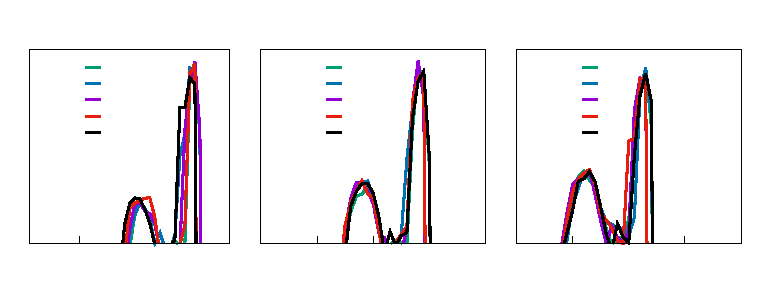
\includegraphics{zif8x-pores-sizes}}%
    \gplfronttext
  \end{picture}%
\endgroup

    \caption{Pore size distribution (no unit) under increasing loading for the
    three structures.}
    \label{fig:zif8x:pores-sizes}
\end{figure}

\begin{figure}[b]
    \centering
    % GNUPLOT: LaTeX picture with Postscript
\begingroup
  \makeatletter
  \providecommand\color[2][]{%
    \GenericError{(gnuplot) \space\space\space\@spaces}{%
      Package color not loaded in conjunction with
      terminal option `colourtext'%
    }{See the gnuplot documentation for explanation.%
    }{Either use 'blacktext' in gnuplot or load the package
      color.sty in LaTeX.}%
    \renewcommand\color[2][]{}%
  }%
  \providecommand\includegraphics[2][]{%
    \GenericError{(gnuplot) \space\space\space\@spaces}{%
      Package graphicx or graphics not loaded%
    }{See the gnuplot documentation for explanation.%
    }{The gnuplot epslatex terminal needs graphicx.sty or graphics.sty.}%
    \renewcommand\includegraphics[2][]{}%
  }%
  \providecommand\rotatebox[2]{#2}%
  \@ifundefined{ifGPcolor}{%
    \newif\ifGPcolor
    \GPcolortrue
  }{}%
  \@ifundefined{ifGPblacktext}{%
    \newif\ifGPblacktext
    \GPblacktextfalse
  }{}%
  % define a \g@addto@macro without @ in the name:
  \let\gplgaddtomacro\g@addto@macro
  % define empty templates for all commands taking text:
  \gdef\gplbacktext{}%
  \gdef\gplfronttext{}%
  \makeatother
  \ifGPblacktext
    % no textcolor at all
    \def\colorrgb#1{}%
    \def\colorgray#1{}%
  \else
    % gray or color?
    \ifGPcolor
      \def\colorrgb#1{\color[rgb]{#1}}%
      \def\colorgray#1{\color[gray]{#1}}%
      \expandafter\def\csname LTw\endcsname{\color{white}}%
      \expandafter\def\csname LTb\endcsname{\color{black}}%
      \expandafter\def\csname LTa\endcsname{\color{black}}%
      \expandafter\def\csname LT0\endcsname{\color[rgb]{1,0,0}}%
      \expandafter\def\csname LT1\endcsname{\color[rgb]{0,1,0}}%
      \expandafter\def\csname LT2\endcsname{\color[rgb]{0,0,1}}%
      \expandafter\def\csname LT3\endcsname{\color[rgb]{1,0,1}}%
      \expandafter\def\csname LT4\endcsname{\color[rgb]{0,1,1}}%
      \expandafter\def\csname LT5\endcsname{\color[rgb]{1,1,0}}%
      \expandafter\def\csname LT6\endcsname{\color[rgb]{0,0,0}}%
      \expandafter\def\csname LT7\endcsname{\color[rgb]{1,0.3,0}}%
      \expandafter\def\csname LT8\endcsname{\color[rgb]{0.5,0.5,0.5}}%
    \else
      % gray
      \def\colorrgb#1{\color{black}}%
      \def\colorgray#1{\color[gray]{#1}}%
      \expandafter\def\csname LTw\endcsname{\color{white}}%
      \expandafter\def\csname LTb\endcsname{\color{black}}%
      \expandafter\def\csname LTa\endcsname{\color{black}}%
      \expandafter\def\csname LT0\endcsname{\color{black}}%
      \expandafter\def\csname LT1\endcsname{\color{black}}%
      \expandafter\def\csname LT2\endcsname{\color{black}}%
      \expandafter\def\csname LT3\endcsname{\color{black}}%
      \expandafter\def\csname LT4\endcsname{\color{black}}%
      \expandafter\def\csname LT5\endcsname{\color{black}}%
      \expandafter\def\csname LT6\endcsname{\color{black}}%
      \expandafter\def\csname LT7\endcsname{\color{black}}%
      \expandafter\def\csname LT8\endcsname{\color{black}}%
    \fi
  \fi
    \setlength{\unitlength}{0.0500bp}%
    \ifx\gptboxheight\undefined%
      \newlength{\gptboxheight}%
      \newlength{\gptboxwidth}%
      \newsavebox{\gptboxtext}%
    \fi%
    \setlength{\fboxrule}{0.5pt}%
    \setlength{\fboxsep}{1pt}%
\begin{picture}(7360.00,2820.00)%
    \gplgaddtomacro\gplbacktext{%
      \csname LTb\endcsname%%
      \put(622,310){\makebox(0,0)[r]{\strut{}$0$}}%
      \csname LTb\endcsname%%
      \put(622,702){\makebox(0,0)[r]{\strut{}$250$}}%
      \csname LTb\endcsname%%
      \put(622,1095){\makebox(0,0)[r]{\strut{}$500$}}%
      \csname LTb\endcsname%%
      \put(622,1487){\makebox(0,0)[r]{\strut{}$750$}}%
      \csname LTb\endcsname%%
      \put(622,1879){\makebox(0,0)[r]{\strut{}$1000$}}%
      \csname LTb\endcsname%%
      \put(622,2272){\makebox(0,0)[r]{\strut{}$1250$}}%
      \csname LTb\endcsname%%
      \put(622,2664){\makebox(0,0)[r]{\strut{}$1500$}}%
      \csname LTb\endcsname%%
      \put(1773,155){\makebox(0,0){\strut{}\ZIF8}}%
      \csname LTb\endcsname%%
      \put(3906,155){\makebox(0,0){\strut{}\ZIFCl}}%
      \csname LTb\endcsname%%
      \put(6038,155){\makebox(0,0){\strut{}\ZIFBr}}%
      \csname LTb\endcsname%%
      \put(1027,2334){\makebox(0,0)[l]{\strut{}\scriptsize 0}}%
      \csname LTb\endcsname%%
      \put(1347,2350){\makebox(0,0)[l]{\strut{}\scriptsize 10}}%
      \csname LTb\endcsname%%
      \put(1709,2342){\makebox(0,0)[l]{\strut{}\scriptsize 25}}%
      \csname LTb\endcsname%%
      \put(2050,2295){\makebox(0,0)[l]{\strut{}\scriptsize 40}}%
      \csname LTb\endcsname%%
      \put(2413,2256){\makebox(0,0)[l]{\strut{}\scriptsize 50}}%
      \csname LTb\endcsname%%
      \put(3159,2303){\makebox(0,0)[l]{\strut{}\scriptsize 0}}%
      \csname LTb\endcsname%%
      \put(3500,2287){\makebox(0,0)[l]{\strut{}\scriptsize 10}}%
      \csname LTb\endcsname%%
      \put(3842,2311){\makebox(0,0)[l]{\strut{}\scriptsize 25}}%
      \csname LTb\endcsname%%
      \put(4183,2319){\makebox(0,0)[l]{\strut{}\scriptsize 40}}%
      \csname LTb\endcsname%%
      \put(4545,2232){\makebox(0,0)[l]{\strut{}\scriptsize 50}}%
      \csname LTb\endcsname%%
      \put(5292,2138){\makebox(0,0)[l]{\strut{}\scriptsize 0}}%
      \csname LTb\endcsname%%
      \put(5654,2154){\makebox(0,0)[l]{\strut{}\scriptsize 8}}%
      \csname LTb\endcsname%%
      \put(5995,2141){\makebox(0,0)[l]{\strut{}\scriptsize 20}}%
      \csname LTb\endcsname%%
      \put(6315,2173){\makebox(0,0)[l]{\strut{}\scriptsize 40}}%
      \csname LTb\endcsname%%
      \put(6678,2130){\makebox(0,0)[l]{\strut{}\scriptsize 50}}%
    }%
    \gplgaddtomacro\gplfronttext{%
      \csname LTb\endcsname%%
      \put(42,1487){\rotatebox{-270}{\makebox(0,0){\strut{}\footnotesize porous volume ($\AA^3$)}}}%
    }%
    \gplbacktext
    \put(0,0){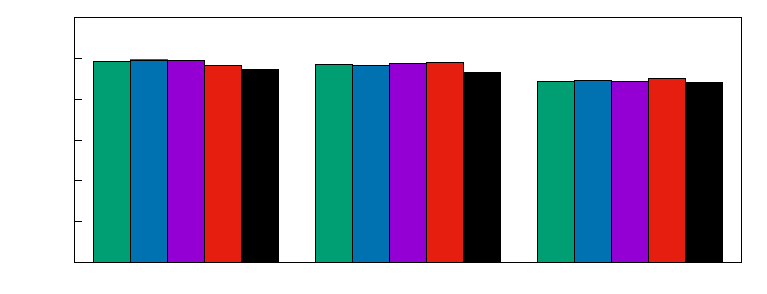
\includegraphics{zif8x-porous-volume}}%
    \gplfronttext
  \end{picture}%
\endgroup

    \caption{Accessible porous volume changes in the three isoreticular
    structures during adsorption. The numbers on top of the columns are the
    number of adsorbed \ce{N2} molecules.}
    \label{fig:zif8x:porous-volume}
\end{figure}

Although this behavior appears to be correlated with the presence or absence of
the adsorption step in the isotherms, it is not however sufficient to explain
it. A first hypothesis to understand the link between linkers swing and the
isotherms step is that the swinging motion could lead to an increase of the
accessible porous volume in the structure, thereby increasing nitrogen uptake.
In order to check whether this is or not the case, I computed the pore size
distribution (see figure~\ref{fig:zif8x:pores-sizes}) and the accessible porous
volume (see figure~\ref{fig:zif8x:porous-volume}) from the trajectories using
Zeo++\cite{Willems2012} version 0.3. In order to compute these values, I first
emptied the structure of all the nitrogen molecules, and then computed the pores
sizes distribution and accessible volume of the remaining frameworks. The
algorithm used by Zeo++ starts by computing the Voronoï decomposition of the
framework, which provides a representation of the void space in the structure.
Then, it uses Monte Carlo sampling of the Voronoï network to extract the volume
accessible to a probe molecule of a given radius and the pore size distribution.
I used the standard probe radius of \SI{1.2}{\AA}, corresponding to a Helium
atom.

The results presented in figure~\ref{fig:zif8x:pores-sizes} highlight that the
pore size distribution (PSD) remains largely unchanged in all cases as the
loading increase and the linkers swing. The PSDs present two peaks,
corresponding to two types of cavities: a small one corresponding to the 6
member windows around \SI{10.3}{\AA} for \ZIF8 and a second one, with a much
larger contribution to the overall porous volume around \SI{11.2}{\AA} in \ZIF8.
The three PSDs are very similar, only changing in the absolute the size of
pores, in the order $\text{\ZIF8} > \text{\ZIFCl} > \text{\ZIFBr}$. This is also
reflected in the accessible volume figure~\ref{fig:zif8x:porous-volume} which
remains roughly constant as the loading increase and the linkers swing.

\subsection{Changes in the adsorbed phase}

\begin{figure}[ht]
    \centering
    % GNUPLOT: LaTeX picture with Postscript
\begingroup
  \makeatletter
  \providecommand\color[2][]{%
    \GenericError{(gnuplot) \space\space\space\@spaces}{%
      Package color not loaded in conjunction with
      terminal option `colourtext'%
    }{See the gnuplot documentation for explanation.%
    }{Either use 'blacktext' in gnuplot or load the package
      color.sty in LaTeX.}%
    \renewcommand\color[2][]{}%
  }%
  \providecommand\includegraphics[2][]{%
    \GenericError{(gnuplot) \space\space\space\@spaces}{%
      Package graphicx or graphics not loaded%
    }{See the gnuplot documentation for explanation.%
    }{The gnuplot epslatex terminal needs graphicx.sty or graphics.sty.}%
    \renewcommand\includegraphics[2][]{}%
  }%
  \providecommand\rotatebox[2]{#2}%
  \@ifundefined{ifGPcolor}{%
    \newif\ifGPcolor
    \GPcolortrue
  }{}%
  \@ifundefined{ifGPblacktext}{%
    \newif\ifGPblacktext
    \GPblacktextfalse
  }{}%
  % define a \g@addto@macro without @ in the name:
  \let\gplgaddtomacro\g@addto@macro
  % define empty templates for all commands taking text:
  \gdef\gplbacktext{}%
  \gdef\gplfronttext{}%
  \makeatother
  \ifGPblacktext
    % no textcolor at all
    \def\colorrgb#1{}%
    \def\colorgray#1{}%
  \else
    % gray or color?
    \ifGPcolor
      \def\colorrgb#1{\color[rgb]{#1}}%
      \def\colorgray#1{\color[gray]{#1}}%
      \expandafter\def\csname LTw\endcsname{\color{white}}%
      \expandafter\def\csname LTb\endcsname{\color{black}}%
      \expandafter\def\csname LTa\endcsname{\color{black}}%
      \expandafter\def\csname LT0\endcsname{\color[rgb]{1,0,0}}%
      \expandafter\def\csname LT1\endcsname{\color[rgb]{0,1,0}}%
      \expandafter\def\csname LT2\endcsname{\color[rgb]{0,0,1}}%
      \expandafter\def\csname LT3\endcsname{\color[rgb]{1,0,1}}%
      \expandafter\def\csname LT4\endcsname{\color[rgb]{0,1,1}}%
      \expandafter\def\csname LT5\endcsname{\color[rgb]{1,1,0}}%
      \expandafter\def\csname LT6\endcsname{\color[rgb]{0,0,0}}%
      \expandafter\def\csname LT7\endcsname{\color[rgb]{1,0.3,0}}%
      \expandafter\def\csname LT8\endcsname{\color[rgb]{0.5,0.5,0.5}}%
    \else
      % gray
      \def\colorrgb#1{\color{black}}%
      \def\colorgray#1{\color[gray]{#1}}%
      \expandafter\def\csname LTw\endcsname{\color{white}}%
      \expandafter\def\csname LTb\endcsname{\color{black}}%
      \expandafter\def\csname LTa\endcsname{\color{black}}%
      \expandafter\def\csname LT0\endcsname{\color{black}}%
      \expandafter\def\csname LT1\endcsname{\color{black}}%
      \expandafter\def\csname LT2\endcsname{\color{black}}%
      \expandafter\def\csname LT3\endcsname{\color{black}}%
      \expandafter\def\csname LT4\endcsname{\color{black}}%
      \expandafter\def\csname LT5\endcsname{\color{black}}%
      \expandafter\def\csname LT6\endcsname{\color{black}}%
      \expandafter\def\csname LT7\endcsname{\color{black}}%
      \expandafter\def\csname LT8\endcsname{\color{black}}%
    \fi
  \fi
    \setlength{\unitlength}{0.0500bp}%
    \ifx\gptboxheight\undefined%
      \newlength{\gptboxheight}%
      \newlength{\gptboxwidth}%
      \newsavebox{\gptboxtext}%
    \fi%
    \setlength{\fboxrule}{0.5pt}%
    \setlength{\fboxsep}{1pt}%
\begin{picture}(7360.00,7360.00)%
    \gplgaddtomacro\gplbacktext{%
    }%
    \gplgaddtomacro\gplfronttext{%
      \csname LTb\endcsname%%
      \put(919,7250){\makebox(0,0){\strut{}\small 10 \ce{N2} $\in$ \ZIFCH3}}%
    }%
    \gplgaddtomacro\gplbacktext{%
    }%
    \gplgaddtomacro\gplfronttext{%
      \csname LTb\endcsname%%
      \put(2759,7250){\makebox(0,0){\strut{}\small 25 \ce{N2} $\in$ \ZIFCH3}}%
    }%
    \gplgaddtomacro\gplbacktext{%
    }%
    \gplgaddtomacro\gplfronttext{%
      \csname LTb\endcsname%%
      \put(4599,7250){\makebox(0,0){\strut{}\small 40 \ce{N2} $\in$ \ZIFCH3}}%
    }%
    \gplgaddtomacro\gplbacktext{%
    }%
    \gplgaddtomacro\gplfronttext{%
      \csname LTb\endcsname%%
      \put(6439,7250){\makebox(0,0){\strut{}\small 50 \ce{N2} $\in$ \ZIFCH3}}%
    }%
    \gplgaddtomacro\gplbacktext{%
    }%
    \gplgaddtomacro\gplfronttext{%
      \csname LTb\endcsname%%
      \put(919,4797){\makebox(0,0){\strut{}\small 10 \ce{N2} $\in$ \ZIFCl}}%
    }%
    \gplgaddtomacro\gplbacktext{%
    }%
    \gplgaddtomacro\gplfronttext{%
      \csname LTb\endcsname%%
      \put(2759,4797){\makebox(0,0){\strut{}\small 25 \ce{N2} $\in$ \ZIFCl}}%
    }%
    \gplgaddtomacro\gplbacktext{%
    }%
    \gplgaddtomacro\gplfronttext{%
      \csname LTb\endcsname%%
      \put(4599,4797){\makebox(0,0){\strut{}\small 40 \ce{N2} $\in$ \ZIFCl}}%
    }%
    \gplgaddtomacro\gplbacktext{%
    }%
    \gplgaddtomacro\gplfronttext{%
      \csname LTb\endcsname%%
      \put(6439,4797){\makebox(0,0){\strut{}\small 50 \ce{N2} $\in$ \ZIFCl}}%
    }%
    \gplgaddtomacro\gplbacktext{%
    }%
    \gplgaddtomacro\gplfronttext{%
      \csname LTb\endcsname%%
      \put(919,2344){\makebox(0,0){\strut{}\small 8 \ce{N2} $\in$ \ZIFBr}}%
    }%
    \gplgaddtomacro\gplbacktext{%
    }%
    \gplgaddtomacro\gplfronttext{%
      \csname LTb\endcsname%%
      \put(2759,2344){\makebox(0,0){\strut{}\small 20 \ce{N2} $\in$ \ZIFBr}}%
    }%
    \gplgaddtomacro\gplbacktext{%
    }%
    \gplgaddtomacro\gplfronttext{%
      \csname LTb\endcsname%%
      \put(4599,2344){\makebox(0,0){\strut{}\small 40 \ce{N2} $\in$ \ZIFBr}}%
    }%
    \gplgaddtomacro\gplbacktext{%
    }%
    \gplgaddtomacro\gplfronttext{%
      \csname LTb\endcsname%%
      \put(6439,2344){\makebox(0,0){\strut{}\small 50 \ce{N2} $\in$ \ZIFBr}}%
    }%
    \gplbacktext
    \put(0,0){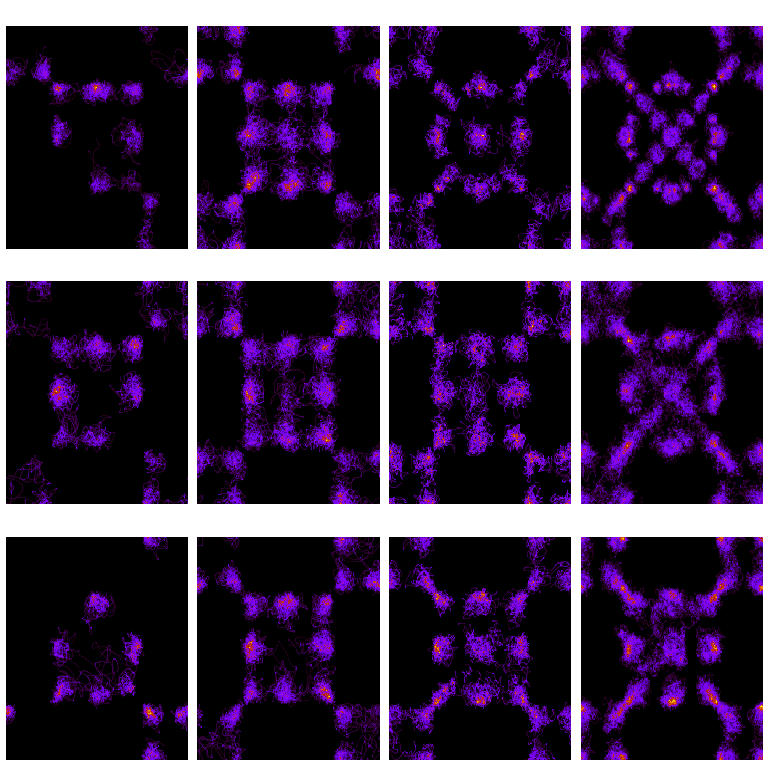
\includegraphics{zif8x-density}}%
    \gplfronttext
  \end{picture}%
\endgroup

    \caption{2D density maps of the adsorbed nitrogen atoms positions in the $xy$
    plane at various loadings in \ZIF8 (top), \ZIFCl (middle), and \ZIFBr
    (bottom). The loading increases from left to right.}
    \label{fig:zif8x:density}
\end{figure}

The hypothesis that the linkers swing leads to an increase of the accessible
porous volume in the structure does not seem to be able to explain the stepped
adsorption isotherm. We need now to take a look at the other chemical species
participating in adsorption: the nitrogen fluid. Another hypothesis we can
formulate to explain the stepped isotherm is that nitrogen molecules undergo a
reordering or repacking in the cavity, thereby leading to an increase in
adsorbed molecules in the same total pore volume as well as the swing of the
linkers aiming to accommodate the new packing. This has already been proposed by
\citeauthor{Ania2012}\cite{Ania2012}, but the intermediate adsorption regime was
not probed or interpreted.In order to visualize this packing, I have projected
the positions of all adsorbed nitrogen atoms in the $xy$ plane and created a
density map of the adsorbed phase. This density map is shown
figure~\ref{fig:zif8x:density} both at various loadings and for the three
frameworks.

\begin{figure}[t]
    \centering
    % GNUPLOT: LaTeX picture with Postscript
\begingroup
  \makeatletter
  \providecommand\color[2][]{%
    \GenericError{(gnuplot) \space\space\space\@spaces}{%
      Package color not loaded in conjunction with
      terminal option `colourtext'%
    }{See the gnuplot documentation for explanation.%
    }{Either use 'blacktext' in gnuplot or load the package
      color.sty in LaTeX.}%
    \renewcommand\color[2][]{}%
  }%
  \providecommand\includegraphics[2][]{%
    \GenericError{(gnuplot) \space\space\space\@spaces}{%
      Package graphicx or graphics not loaded%
    }{See the gnuplot documentation for explanation.%
    }{The gnuplot epslatex terminal needs graphicx.sty or graphics.sty.}%
    \renewcommand\includegraphics[2][]{}%
  }%
  \providecommand\rotatebox[2]{#2}%
  \@ifundefined{ifGPcolor}{%
    \newif\ifGPcolor
    \GPcolortrue
  }{}%
  \@ifundefined{ifGPblacktext}{%
    \newif\ifGPblacktext
    \GPblacktextfalse
  }{}%
  % define a \g@addto@macro without @ in the name:
  \let\gplgaddtomacro\g@addto@macro
  % define empty templates for all commands taking text:
  \gdef\gplbacktext{}%
  \gdef\gplfronttext{}%
  \makeatother
  \ifGPblacktext
    % no textcolor at all
    \def\colorrgb#1{}%
    \def\colorgray#1{}%
  \else
    % gray or color?
    \ifGPcolor
      \def\colorrgb#1{\color[rgb]{#1}}%
      \def\colorgray#1{\color[gray]{#1}}%
      \expandafter\def\csname LTw\endcsname{\color{white}}%
      \expandafter\def\csname LTb\endcsname{\color{black}}%
      \expandafter\def\csname LTa\endcsname{\color{black}}%
      \expandafter\def\csname LT0\endcsname{\color[rgb]{1,0,0}}%
      \expandafter\def\csname LT1\endcsname{\color[rgb]{0,1,0}}%
      \expandafter\def\csname LT2\endcsname{\color[rgb]{0,0,1}}%
      \expandafter\def\csname LT3\endcsname{\color[rgb]{1,0,1}}%
      \expandafter\def\csname LT4\endcsname{\color[rgb]{0,1,1}}%
      \expandafter\def\csname LT5\endcsname{\color[rgb]{1,1,0}}%
      \expandafter\def\csname LT6\endcsname{\color[rgb]{0,0,0}}%
      \expandafter\def\csname LT7\endcsname{\color[rgb]{1,0.3,0}}%
      \expandafter\def\csname LT8\endcsname{\color[rgb]{0.5,0.5,0.5}}%
    \else
      % gray
      \def\colorrgb#1{\color{black}}%
      \def\colorgray#1{\color[gray]{#1}}%
      \expandafter\def\csname LTw\endcsname{\color{white}}%
      \expandafter\def\csname LTb\endcsname{\color{black}}%
      \expandafter\def\csname LTa\endcsname{\color{black}}%
      \expandafter\def\csname LT0\endcsname{\color{black}}%
      \expandafter\def\csname LT1\endcsname{\color{black}}%
      \expandafter\def\csname LT2\endcsname{\color{black}}%
      \expandafter\def\csname LT3\endcsname{\color{black}}%
      \expandafter\def\csname LT4\endcsname{\color{black}}%
      \expandafter\def\csname LT5\endcsname{\color{black}}%
      \expandafter\def\csname LT6\endcsname{\color{black}}%
      \expandafter\def\csname LT7\endcsname{\color{black}}%
      \expandafter\def\csname LT8\endcsname{\color{black}}%
    \fi
  \fi
    \setlength{\unitlength}{0.0500bp}%
    \ifx\gptboxheight\undefined%
      \newlength{\gptboxheight}%
      \newlength{\gptboxwidth}%
      \newsavebox{\gptboxtext}%
    \fi%
    \setlength{\fboxrule}{0.5pt}%
    \setlength{\fboxsep}{1pt}%
\begin{picture}(4520.00,5660.00)%
    \gplgaddtomacro\gplbacktext{%
      \csname LTb\endcsname%%
      \put(1568,3928){\makebox(0,0){\strut{}$0$}}%
      \csname LTb\endcsname%%
      \put(1953,3928){\makebox(0,0){\strut{}$1$}}%
      \csname LTb\endcsname%%
      \put(2338,3928){\makebox(0,0){\strut{}$2$}}%
      \csname LTb\endcsname%%
      \put(2723,3928){\makebox(0,0){\strut{}$3$}}%
      \csname LTb\endcsname%%
      \put(3109,3928){\makebox(0,0){\strut{}$4$}}%
      \csname LTb\endcsname%%
      \put(3494,3928){\makebox(0,0){\strut{}$5$}}%
      \csname LTb\endcsname%%
      \put(3879,3928){\makebox(0,0){\strut{}$6$}}%
      \csname LTb\endcsname%%
      \put(4264,3928){\makebox(0,0){\strut{}$7$}}%
      \csname LTb\endcsname%%
      \put(490,4794){\makebox(0,0)[l]{\strut{}\small \ZIFCH3}}%
    }%
    \gplgaddtomacro\gplfronttext{%
      \csname LTb\endcsname%%
      \put(2329,5355){\makebox(0,0)[r]{\strut{}\scriptsize 10 \ce{N2}}}%
      \csname LTb\endcsname%%
      \put(2329,5200){\makebox(0,0)[r]{\strut{}\scriptsize 25 \ce{N2}}}%
      \csname LTb\endcsname%%
      \put(2329,5045){\makebox(0,0)[r]{\strut{}\scriptsize 40 \ce{N2}}}%
      \csname LTb\endcsname%%
      \put(2329,4890){\makebox(0,0)[r]{\strut{}\scriptsize 50 \ce{N2}}}%
    }%
    \gplgaddtomacro\gplbacktext{%
      \csname LTb\endcsname%%
      \put(1568,2041){\makebox(0,0){\strut{}$0$}}%
      \csname LTb\endcsname%%
      \put(1953,2041){\makebox(0,0){\strut{}$1$}}%
      \csname LTb\endcsname%%
      \put(2338,2041){\makebox(0,0){\strut{}$2$}}%
      \csname LTb\endcsname%%
      \put(2723,2041){\makebox(0,0){\strut{}$3$}}%
      \csname LTb\endcsname%%
      \put(3109,2041){\makebox(0,0){\strut{}$4$}}%
      \csname LTb\endcsname%%
      \put(3494,2041){\makebox(0,0){\strut{}$5$}}%
      \csname LTb\endcsname%%
      \put(3879,2041){\makebox(0,0){\strut{}$6$}}%
      \csname LTb\endcsname%%
      \put(4264,2041){\makebox(0,0){\strut{}$7$}}%
      \csname LTb\endcsname%%
      \put(490,2907){\makebox(0,0)[l]{\strut{}\small \ZIFCl}}%
    }%
    \gplgaddtomacro\gplfronttext{%
      \csname LTb\endcsname%%
      \put(2329,3469){\makebox(0,0)[r]{\strut{}\scriptsize 10 \ce{N2}}}%
      \csname LTb\endcsname%%
      \put(2329,3314){\makebox(0,0)[r]{\strut{}\scriptsize 25 \ce{N2}}}%
      \csname LTb\endcsname%%
      \put(2329,3159){\makebox(0,0)[r]{\strut{}\scriptsize 40 \ce{N2}}}%
      \csname LTb\endcsname%%
      \put(2329,3004){\makebox(0,0)[r]{\strut{}\scriptsize 50 \ce{N2}}}%
    }%
    \gplgaddtomacro\gplbacktext{%
      \csname LTb\endcsname%%
      \put(1568,155){\makebox(0,0){\strut{}$0$}}%
      \csname LTb\endcsname%%
      \put(1953,155){\makebox(0,0){\strut{}$1$}}%
      \csname LTb\endcsname%%
      \put(2338,155){\makebox(0,0){\strut{}$2$}}%
      \csname LTb\endcsname%%
      \put(2723,155){\makebox(0,0){\strut{}$3$}}%
      \csname LTb\endcsname%%
      \put(3109,155){\makebox(0,0){\strut{}$4$}}%
      \csname LTb\endcsname%%
      \put(3494,155){\makebox(0,0){\strut{}$5$}}%
      \csname LTb\endcsname%%
      \put(3879,155){\makebox(0,0){\strut{}$6$}}%
      \csname LTb\endcsname%%
      \put(4264,155){\makebox(0,0){\strut{}$7$}}%
      \csname LTb\endcsname%%
      \put(490,1021){\makebox(0,0)[l]{\strut{}\small \ZIFBr}}%
    }%
    \gplgaddtomacro\gplfronttext{%
      \csname LTb\endcsname%%
      \put(2329,1582){\makebox(0,0)[r]{\strut{}\scriptsize 8 \ce{N2}}}%
      \csname LTb\endcsname%%
      \put(2329,1427){\makebox(0,0)[r]{\strut{}\scriptsize 20 \ce{N2}}}%
      \csname LTb\endcsname%%
      \put(2329,1272){\makebox(0,0)[r]{\strut{}\scriptsize 40 \ce{N2}}}%
      \csname LTb\endcsname%%
      \put(2329,1117){\makebox(0,0)[r]{\strut{}\scriptsize 50 \ce{N2}}}%
    }%
    \gplbacktext
    \put(0,0){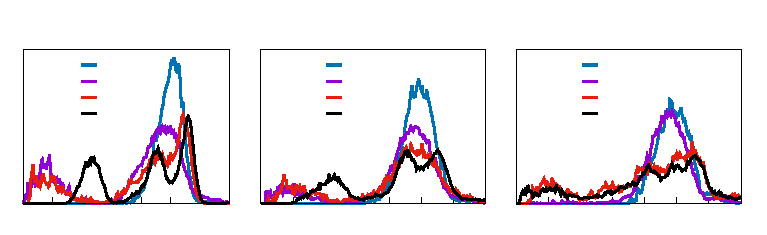
\includegraphics{zif8x-rdf}}%
    \gplfronttext
  \end{picture}%
\endgroup

    \caption{Radial distribution function of nitrogen atoms in the three
    frameworks for various nitrogen loading. This represent the number of atoms
    at a given distance from the center of the cavity.}
    \label{fig:zif8x:rdf}
\end{figure}

For \ZIFCH3, two different molecular packing are encountered according to the
loading. With 10 or 25 molecules in the unit cell, the density maps show clear
delimited positions on a cubic-like arrangement, whereas with 40 and 50
molecules, they show a tetragonal-like arrangement of the molecules. This
reordering of the adsorbed nitrogen molecules from a cubic-like phase to a
tetragonal-like phase is at the origin of the steep uptake at low relative
pressure. For \ZIFCl, the behavior is roughly similar: the molecules first pack
in a cubic-like fashion in the cases of 10, 25 and 40 molecules per unit cell,
before a reordering toward a tetragonal-like arrangement at 50 molecules per
unit cell. This is consistent with the dihedral angles distributions as shown in
figure~\ref{fig:zif8x:dihedrals}, and evidence that the molecular packing
rearrangement happens conjointly with the swing of the linkers. It is
interesting to note that some disorder in the tetragonal arrangement remains ---
even at a loading of 50 molecules per unit cell --- as the molecules' positions
are not as well defined as the one in \ZIF8. Again, this is consistent with the
dihedral angles distribution at 50 molecules per unit cell for \ZIFCl which is
not of a single Gaussian type, indicating that this disorder can also be found
in the framework structure. For \ZIFBr, the behavior is different. A same
cubic-like arrangement is found at the lower loadings of 8 and 20 molecules per
unit cell, whereas the arrangement at the higher loadings of 40 and 50 molecules
per cell differs from the tetragonal-like one seen for \ZIF8 and \ZIFCl. Indeed,
the latter appears as a mix of the cubic and the tetragonal organization as the
molecules are mostly distributed on a cube with additional molecules in the
[111] channels on the diagonals of the cube. Consequently, because of the
absence of a clear reordering of adsorbed nitrogen molecules in \ZIFBr, its
sorption isotherm does not display the S-shaped adsorption step.

This repacking of nitrogen molecules is also visible on the radial distribution
of nitrogen atoms (not to be confused with the pairs radial distribution
function $g(r)$) in figure~\ref{fig:zif8x:rdf}. The radial distribution counts
how many nitrogen atoms are at a given distance from the center of the sodalite
cage. On the graphs for the \ZIF8 framework, we can see the change from the
initial packing at $N = 10$ and $N = 25$ with a main peak at \SI{5}{\AA} and a
secondary peak at \SI{1}{\AA}; the final packing at $N = 50$ with three well
defined peaks at \SI{2.5}{\AA}, \SI{4.5}{\AA}, and \SI{5.5}{\AA}; and the $N =
40$ distribution which present characteristics of both extremes. Again, for
\ZIFCl, we observe the first bi-modal distribution for $N = 10$, 25 and 40; and
the tri-modal distribution for $N = 50$. And in \ZIFBr we never see the
tri-modal distribution: instead at high loadings ($N = 40$ and $N = 50$) the
curve is not well defined in the 3 to \SI{6}{\AA} range, as already seen in
figure~\ref{fig:zif8x:density}.

\subsection{Mechanism of nitrogen adsorption in \ZIF8}

\begin{figure}[ht]
    \centering
    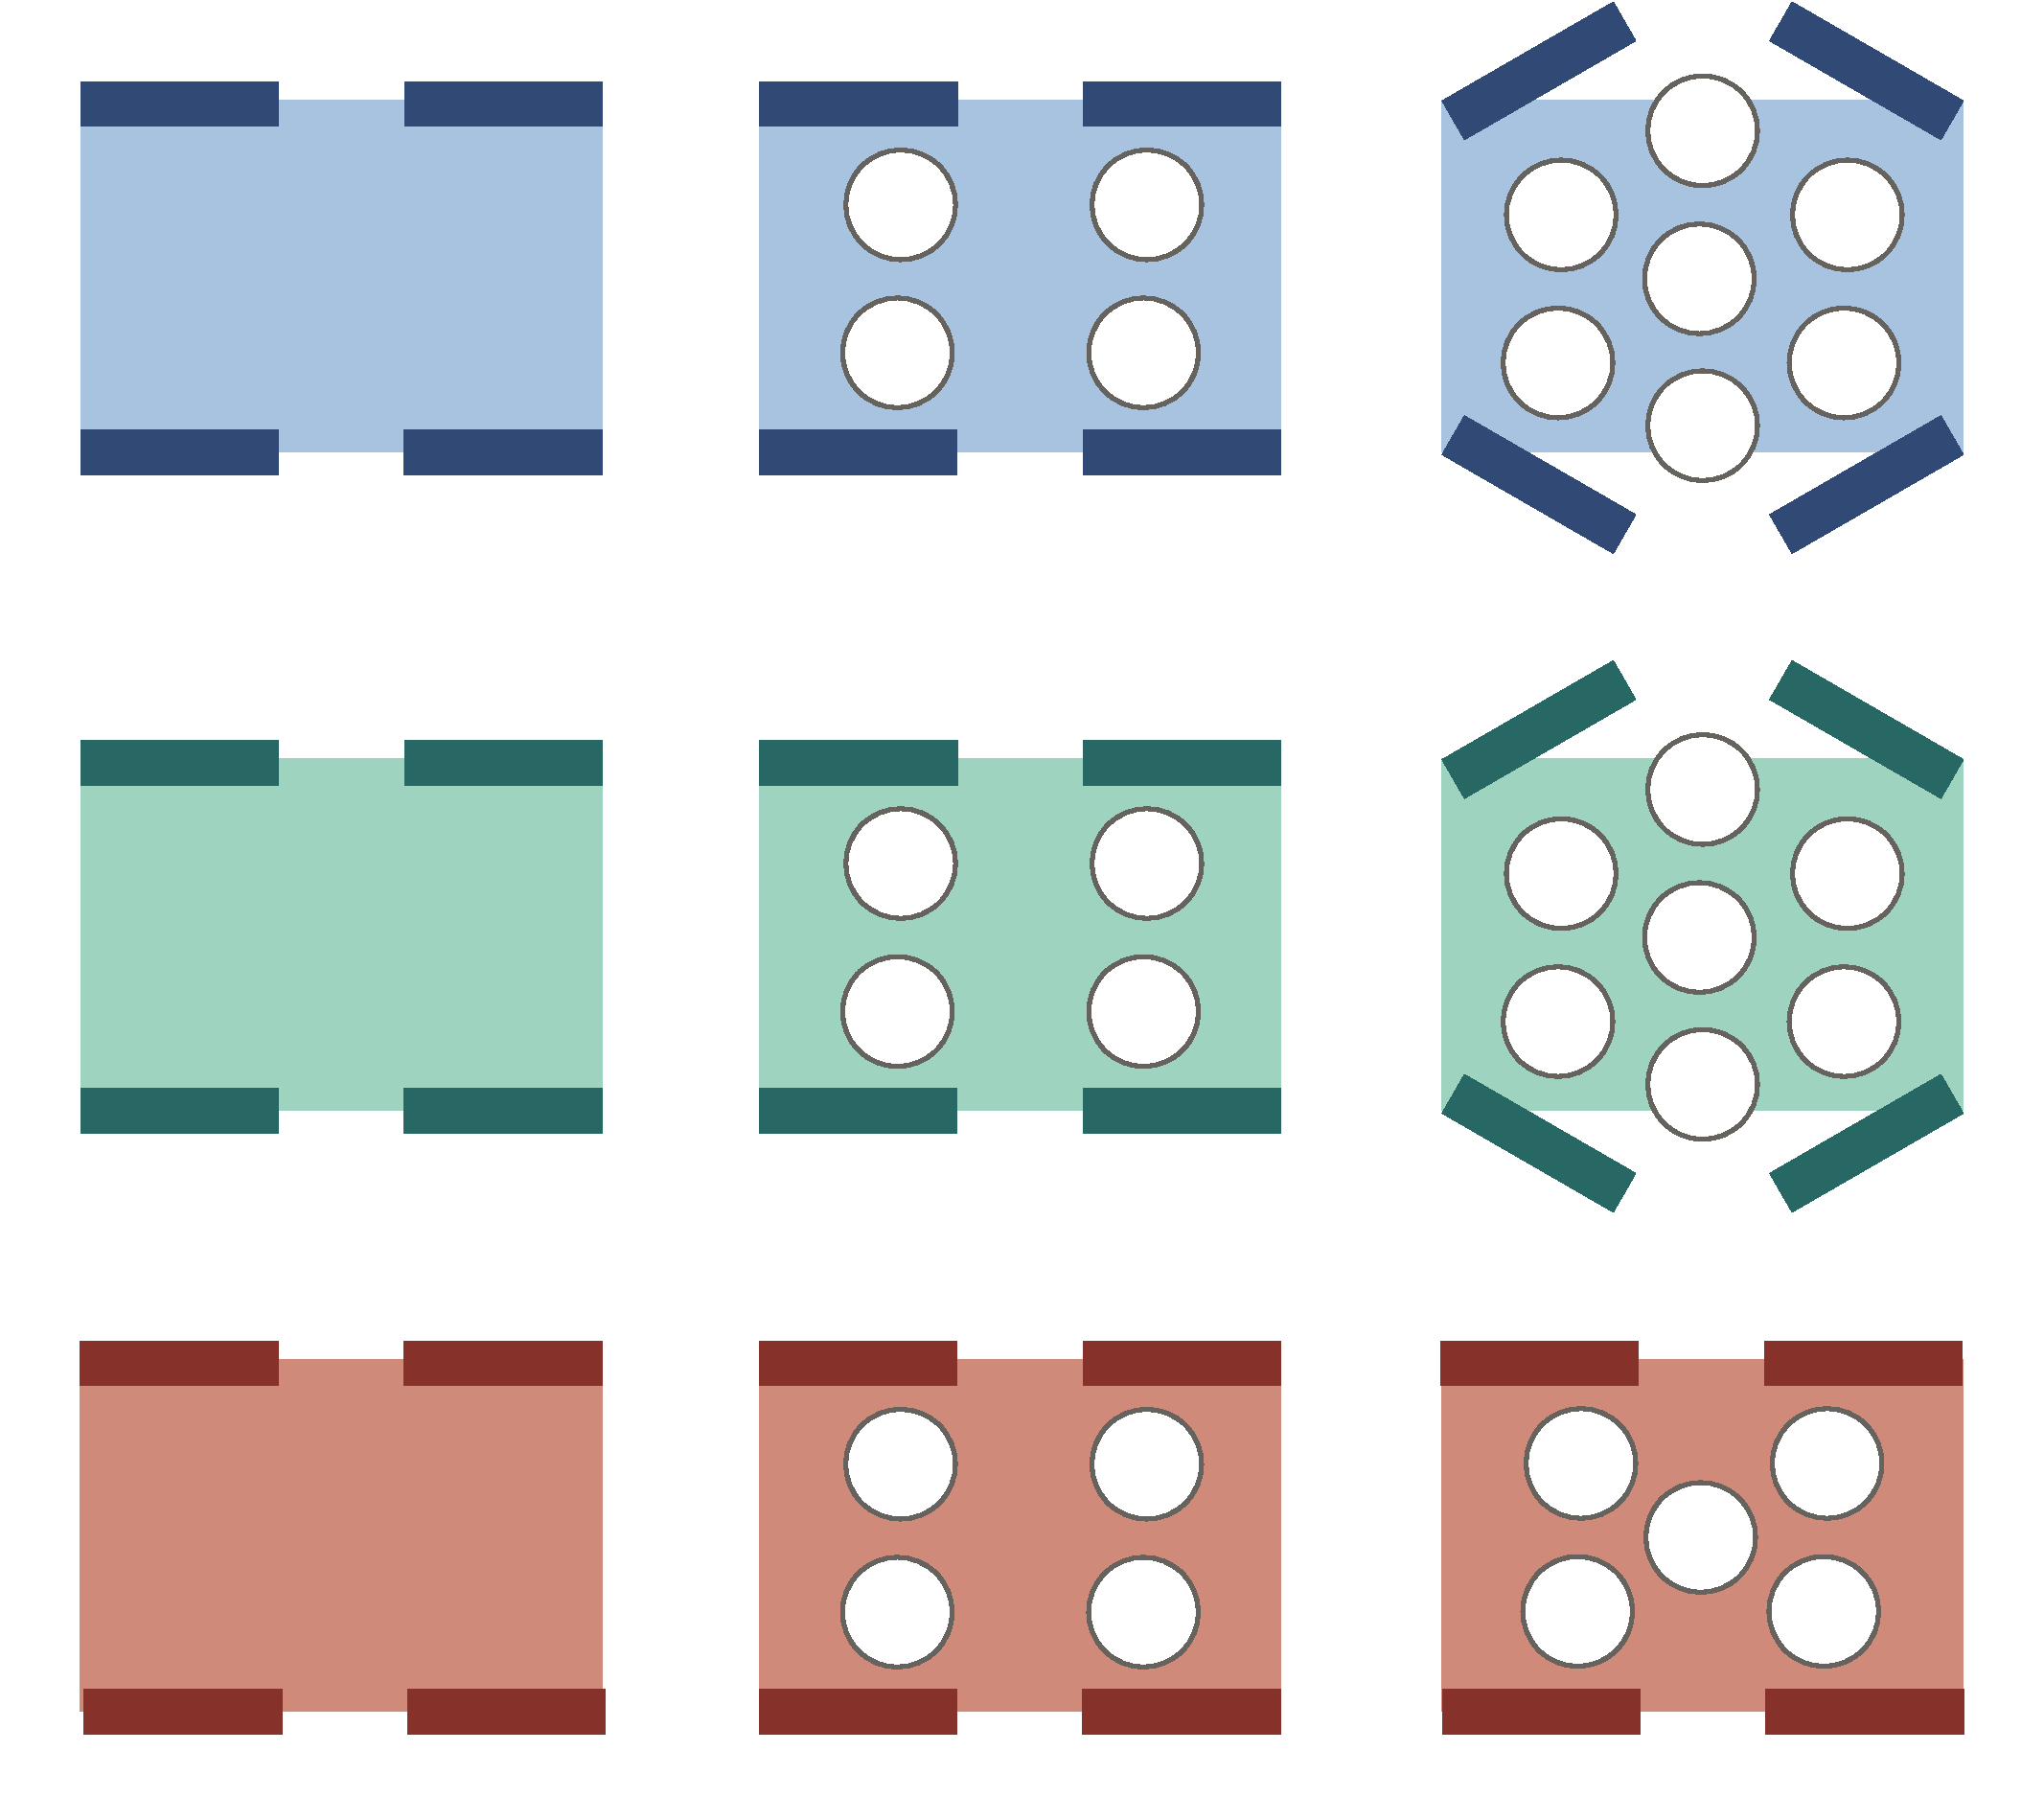
\includegraphics[width=0.5\textwidth]{figures/images/zif8x-summary}
    \caption{Schematic overview of the adsorption process in the three \ZIF8
    frameworks. Blue is \ZIFCH3, green is \ZIFCl and red is \ZIFBr; loading
    increases from left to right.}
    \label{fig:zif8x:summary}
\end{figure}

To summarize this section, the proposed mechanism of nitrogen adsorption in the
three \ZIF8 frameworks with different functionalization is illustrated in a
schematic way in figure~\ref{fig:zif8x:summary}. When the pores are empty, the
linkers are in their equilibrium position, around 0°. As the loading increases,
the pores start to fill in a given, cubic-like arrangement. Then, as loading
continues to increase, in \ZIFCH3 and \ZIFCl the nitrogen molecules arrangement
changes to a tetragonal-like arrangement and the linkers rotate to accommodate
for this repacking. In \ZIFBr, the nitrogen molecules do not repack and the
linkers do not rotate.

Given that the change in functional group from methyl to chloro and bromo does
not significantly impact partial atomic charges or the strength of the \ce{Zn-N}
coordination bond, the origin of the different sorption features between the
three \ZIF8 derivatives does not come from a difference in flexibility or
stiffness of the linkers rotation. This is confirmed by the dihedral angles
distribution in figure~\ref{fig:zif8x:dihedrals}, where all the Gaussian
distributions have the same width, which means that all the linkers rotation
have the same stiffness. Instead, the differences in the adsorption isotherms
come from the differences in pore size and shape, the pores in \ZIFBr being
smaller than in \ZIFCl and \ZIFCH3, thus preventing a molecular reordering to
occur.

\section{Classical force fields from \abinitio data}
\label{sec:classical-ff-parametrize}

As mentioned in section~\ref{sec:zif8x:methods}, I used \abinitio molecular
dynamics to study the adsorption in the three \ZIF8 derivatives to be able to
describe the full flexibility of the frameworks without making any other
assumptions; and because there was no available force field for the studied
materials. During my PhD, I have also started a collaboration with Johannes
Dürholt and Rochus Schmid from the Ruhr Universität in Bochum, Germany to
parametrize a classical force field for \ZIFCH3, \ZIFCl, and \ZIFBr using data
from the \abinitio simulations presented above. The corresponding work is
published in \citejournal{Duerholt2019}\cite{Duerholt2019}.

\subsection{Fitting a force field}

Classical force fields are fully defined by two things: (1) the choice of
functional forms used to represent the different terms (\emph{e.g.} using
Lennard-Jones, Buckingham or another form for non-bonded pair interactions), and
(2) the atom-dependent parameters used in these functional forms (like the
$\epsilon$ and $\sigma$ parameters for Lennard-Jones). See
section~\ref{sec:classical-ff} for a more complete description of force fields
and their use in computational chemistry. The process of optimizing the
parameters of a force-field is called the parametrization of the force field.
The idea is to use some reference data, either from experimental properties or
\abinitio computations, and optimize the parameters to reproduce the reference
data in the best possible way. Both static properties such as crystalline
structure from X-ray diffraction, and dynamic ones such as vibrations
frequencies as given by infrared spectroscopy can be used as reference data when
fitting a force field. The created force field can then be evaluated by checking
how well it can reproduce physical properties that were not used for creating it
--- for example the melting point, or solvation energy. A good force field will
be able to reproduce most properties of a system reasonably well.

Historically, optimizing the parameters of a force-field has most often been a
manual and ad hoc process. First, we would start by setting the parameters to an
initial value by making an educated guess, then we would run a few static or
dynamic calculations with these parameters, compute and compare the properties
of interest with the reference value, and finally we would adjust the parameters
and start over, until some convergence was achieved. Convergence is measured by
a cost function that we try to minimize when changing the parameters. Creating a
force field this way is difficult and takes a lot of time. Additionally, it is
not reproducible: starting the process all over again might lead to a different
set of parameters.

\subsubsection{Transferable or accurate?}

Ideally, we want the force fields we use to be as accurate as possible when
computing the energy of a system, to be as confident as possible that the model
described by the force field describe the chemical reality as well as possible.
This means creating a specific force field for every molecule, and for every
combination of molecules. However, having separate force fields for each system
we are interested in can prevent us to compare the predicted properties. We can
not ascribe with certainty the predicted differences to the underlying chemical
reality, and not the model we used. The origin of the discrepancies might also
be the use of different reference data or different functional forms, as well as
a different parametrization procedure.

This is the reason why generic force fields have also been developed. They
trade some accuracy for a better transferability: we are able to use them for
multiple molecular systems with roughly the same accuracy everywhere. The
Universal Force Field\cite{Rappe1992} (UFF) and the AMBER family\cite{Wang2004}
of force fields for bio-molecules are well-known examples of such generic force
fields. Instead of defining a force field for a whole molecule, they are based
on \emph{fragments}. For example methanoic acid \ce{HCOOH} would contain
\ce{C-H}, \ce{C-O}, \ce{C=O}, and \ce{O-H} bond fragments; as well as
\ce{H-C=O}, \ce{O-C=O}, \ce{C-O-H} angles and \ce{O=C-O-H} dihedral angle. The
same fragments would also be used in ethanoic acid \ce{CH3COOH}, or any other
carboxylic acid.

Existing generic force fields are not always optimal for simulating MOFs, mainly
because of the coordination bonds existing between the metallic centers and the
organic linkers. As metal centers are relatively rare in bio-molecules, the
interactions between them and organic molecules are not well described by
existing force fields such as the ones in AMBER family. There also have been
adaptations of UFF for MOFs\cite{Addicoat2014, Coupry2016}, that are able to
reproduce static properties within 10\% for most of the structures. However,
reproducing dynamics properties and especially the flexibility of MOFs is harder.

\subsection{Systematic parametrization of force fields}

One way to overcome the previously mentioned issues (long parametrization time,
non-reproducible parametrization, trade-off between transferable and accurate
force fields) is to use a systematic parametrization algorithm. Using an
algorithm will improve the parametrization time although the generated force
field should still be validated. We can also design the algorithm to give us
reproducible parametrization. Finally, using the same algorithm for all the
systems of interest should help with accuracy --- as each system has parameters
specifically fitted for it --- while still allowing comparison between different
systems because they would share the functional form and kind of input data with
all the other systems.

Several approaches have been developed to generate new force fields for MOFs,
such as Quick-FF\cite{Vanduyfhuys2015} and MOF-FF\cite{Bureekaew2013}. Both
use \abinitio reference data, such as the optimized geometry of the system, and
the Hessian matrix at this optimized geometry; usually represented on a base on
internal coordinates. The Hessian matrix $H$ contains the second derivatives of
the energy with respect to two internal coordinates. To optimize the
parameters, they use machine learning algorithms, such as genetic algorithms.
Genetic algorithms start from a population of randomly created parameter sets,
evaluate a cost function to rank them all. Then --- mimicking evolution
and natural selection --- the weakest sets (the ones with the highest cost) are
eliminated, and the remaining sets are combined to create a new generation of
parameters set. New generations are created until the cost function is minimal
over the whole generation. In this last generation, the best parameter set is
set to be the new force field.

MOF-FF is based on the MM3 functional form\cite{Allinger1989}, and some of the
parameters are fixed before starting the optimization. In particular, atomic
charges are computed directly from the \abinitio reference and represented as
atom-centered spherical Gaussians, while the dispersion interaction is modeled
with a Buckingham potential, using the tabulated parameters for
MM3\cite{Allinger1994}. The remaining intra-molecular parameters are optimized
in order to make sure the overall potential reproduces the reference data. The
score function $Z$ used for optimization is defined for a parameter set $P$ as:
\[
\begin{aligned}
    Z(P) &= \alpha_\text{bonds} \sum_\text{bonds} w_i \ \left[r_i\,(P) - r_i^{ref}\right]^2 \\
         &+ \alpha_\text{dihedrals} \sum_\text{dihedrals} w_i \ \left[\phi_i\,(P) - \phi_i^{ref}\right]^2 \\
         &+ \alpha_\text{diag} \sum_m w_{mm} \ \left[H_{mm}(P) - H_{mm}^{ref}\right]^2 \\
         &+ \frac 1 9 \sum \left[C^{-1} \cdot (S \cdot V)^2\right]^2 \\
\end{aligned}
\begin{aligned}
    &+ \alpha_\text{angles} \sum_\text{angles} w_i \ \left[\theta_i\,(P) - \theta_i^{ref}\right]^2 \\
    &+ \alpha_\text{impropers} \sum_\text{impropers} w_i \ \left[\delta_i\,(P) - \delta_i^{ref}\right]^2 \\
    &+ \alpha_\text{non-diag} \sum_k \sum_{m\neq k} w_{km} \ \left[H_{km}(P) - H_{km}^{ref}\right]^2 \\
    &~
\end{aligned}
\]

All terms are squared mean deviations, weighted both by $w_i$ to set the relative
importance of similar terms; and $\alpha_x$ to set the relative importance of
different terms. The first four terms account for equilibrium values of
geometric parameters, the following two account for the diagonal and out of
diagonal contributions to the Hessian of the system, \ie the dynamics of the
system around equilibrium. The last term contains the unit cell matrix $C$, the
stress $S$ and the unit cell volume $V$, and is used to minimize the resulting
total stress on the periodic system.

Johannes Dürholt used MOF-FF to generate new force fields for \ZIFCH3, \ZIFCl,
and \ZIFBr from \abinitio input data. I contributed to this work by providing
the previously described simulations of empty ZIFs; and by helping to run
analysis on the trajectories in order to validate the force field. Previous
versions of MOF-FF used finite representative clusters in vacuum to parametrize
the force field. During this work, the fitting strategy was improved to allow
the use of periodic boundary conditions in the reference data. This removes the
need to find representative and charge neutral finite clusters, which is not
always possible depending on the MOF topology. Interested readers should refer to
the corresponding article\cite{Duerholt2019} for more information and the force
field parameters.

\subsection{Validating the generated force-fields}

After generating the force field, we ran multiple classical simulations to
validate it. We first checked the static properties of an energy-minimized
structure, starting with the unit cell lattice parameters, reported in
table~\ref{tab:mof-ff:unit-cell}. MOF-FF is able to reproduce very well the DFT
reference used to parametrize it. Since we did not use lattice parameters when
optimizing MOF-FF, this was not guaranteed.

\begin{table}[ht]
    \caption{Unit cell lattice parameters for the three \ZIF8-based frameworks,
    comparing the experimental values to DFT and MOF-FF.}
    \label{tab:mof-ff:unit-cell}
    \vskip0.5\baselineskip
    \centering
    \newcolumntype{C}{>{\centering\arraybackslash}X}
    \begin{tabularx}{0.8\textwidth}{l X C C}
        \toprule
                &                        & $a, b, c \ (\AA)$ & $\alpha, \beta, \gamma \text{(°)}$ \\
        \midrule
                & exp\cite{Park2006}     &     16.99         &  90.00   \\
        \ZIFCH3 & DFT                    &     17.03         &  90.00   \\
                & MOF-FF                 &     17.08         &  90.00   \\
        \midrule
                & exp\cite{Chaplais2018} &     17.04         &  90.00   \\
        \ZIFCl  & DFT                    &     17.20         &  90.00   \\
                & MOF-FF                 &     17.21         &  90.00   \\
        \midrule
                & exp\cite{Chaplais2018} &     17.08         &  90.00   \\
        \ZIFBr  & DFT                    &     17.25         &  90.00   \\
                & MOF-FF                 &     17.25         &  90.00   \\
        \bottomrule
    \end{tabularx}
\end{table}

\begin{table}[b]
    \caption{Elastic constants for the three \ZIF8-based frameworks, comparing
    the values computed by MOF-FF and DFT.}
    \label{tab:mof-ff:elastic}
    \vskip0.5\baselineskip
    \centering
    \newcolumntype{C}{>{\centering\arraybackslash}X}
    \begin{tabularx}{0.8\textwidth}{l X C C C}
        \toprule
                &                     & $C_{11}$ (GPa) & $C_{12}$ (GPa) & $C_{44}$ (GPa) \\
        \midrule
        \ZIFCH3 & DFT\cite{Tan2012}   &     11.04      &  8.32          &  0.94          \\
                & MOF-FF              &     8.54       &  6.55          &  0.62          \\
        \midrule
        \ZIFCl  & DFT                 &     9.23       &  7.35          &  0.86          \\
                & MOF-FF              &     9.92       &  7.84          &  0.46          \\
        \midrule
        \ZIFBr  & DFT                 &     10.33      &  8.31          &  0.88          \\
                & MOF-FF              &     10.51      &  8.65          &  0.19          \\
        \bottomrule
    \end{tabularx}
\end{table}

\begin{figure}[ht]
    \centering
    % GNUPLOT: LaTeX picture with Postscript
\begingroup
  \makeatletter
  \providecommand\color[2][]{%
    \GenericError{(gnuplot) \space\space\space\@spaces}{%
      Package color not loaded in conjunction with
      terminal option `colourtext'%
    }{See the gnuplot documentation for explanation.%
    }{Either use 'blacktext' in gnuplot or load the package
      color.sty in LaTeX.}%
    \renewcommand\color[2][]{}%
  }%
  \providecommand\includegraphics[2][]{%
    \GenericError{(gnuplot) \space\space\space\@spaces}{%
      Package graphicx or graphics not loaded%
    }{See the gnuplot documentation for explanation.%
    }{The gnuplot epslatex terminal needs graphicx.sty or graphics.sty.}%
    \renewcommand\includegraphics[2][]{}%
  }%
  \providecommand\rotatebox[2]{#2}%
  \@ifundefined{ifGPcolor}{%
    \newif\ifGPcolor
    \GPcolortrue
  }{}%
  \@ifundefined{ifGPblacktext}{%
    \newif\ifGPblacktext
    \GPblacktextfalse
  }{}%
  % define a \g@addto@macro without @ in the name:
  \let\gplgaddtomacro\g@addto@macro
  % define empty templates for all commands taking text:
  \gdef\gplbacktext{}%
  \gdef\gplfronttext{}%
  \makeatother
  \ifGPblacktext
    % no textcolor at all
    \def\colorrgb#1{}%
    \def\colorgray#1{}%
  \else
    % gray or color?
    \ifGPcolor
      \def\colorrgb#1{\color[rgb]{#1}}%
      \def\colorgray#1{\color[gray]{#1}}%
      \expandafter\def\csname LTw\endcsname{\color{white}}%
      \expandafter\def\csname LTb\endcsname{\color{black}}%
      \expandafter\def\csname LTa\endcsname{\color{black}}%
      \expandafter\def\csname LT0\endcsname{\color[rgb]{1,0,0}}%
      \expandafter\def\csname LT1\endcsname{\color[rgb]{0,1,0}}%
      \expandafter\def\csname LT2\endcsname{\color[rgb]{0,0,1}}%
      \expandafter\def\csname LT3\endcsname{\color[rgb]{1,0,1}}%
      \expandafter\def\csname LT4\endcsname{\color[rgb]{0,1,1}}%
      \expandafter\def\csname LT5\endcsname{\color[rgb]{1,1,0}}%
      \expandafter\def\csname LT6\endcsname{\color[rgb]{0,0,0}}%
      \expandafter\def\csname LT7\endcsname{\color[rgb]{1,0.3,0}}%
      \expandafter\def\csname LT8\endcsname{\color[rgb]{0.5,0.5,0.5}}%
    \else
      % gray
      \def\colorrgb#1{\color{black}}%
      \def\colorgray#1{\color[gray]{#1}}%
      \expandafter\def\csname LTw\endcsname{\color{white}}%
      \expandafter\def\csname LTb\endcsname{\color{black}}%
      \expandafter\def\csname LTa\endcsname{\color{black}}%
      \expandafter\def\csname LT0\endcsname{\color{black}}%
      \expandafter\def\csname LT1\endcsname{\color{black}}%
      \expandafter\def\csname LT2\endcsname{\color{black}}%
      \expandafter\def\csname LT3\endcsname{\color{black}}%
      \expandafter\def\csname LT4\endcsname{\color{black}}%
      \expandafter\def\csname LT5\endcsname{\color{black}}%
      \expandafter\def\csname LT6\endcsname{\color{black}}%
      \expandafter\def\csname LT7\endcsname{\color{black}}%
      \expandafter\def\csname LT8\endcsname{\color{black}}%
    \fi
  \fi
    \setlength{\unitlength}{0.0500bp}%
    \ifx\gptboxheight\undefined%
      \newlength{\gptboxheight}%
      \newlength{\gptboxwidth}%
      \newsavebox{\gptboxtext}%
    \fi%
    \setlength{\fboxrule}{0.5pt}%
    \setlength{\fboxsep}{1pt}%
\begin{picture}(6800.00,4520.00)%
    \gplgaddtomacro\gplbacktext{%
      \csname LTb\endcsname%%
      \put(470,2685){\makebox(0,0)[r]{\strut{}$1$}}%
      \csname LTb\endcsname%%
      \put(470,2994){\makebox(0,0)[r]{\strut{}$1.2$}}%
      \csname LTb\endcsname%%
      \put(470,3304){\makebox(0,0)[r]{\strut{}$1.4$}}%
      \csname LTb\endcsname%%
      \put(470,3613){\makebox(0,0)[r]{\strut{}$1.6$}}%
      \csname LTb\endcsname%%
      \put(470,3922){\makebox(0,0)[r]{\strut{}$1.8$}}%
      \csname LTb\endcsname%%
      \put(470,4231){\makebox(0,0)[r]{\strut{}$2$}}%
      \csname LTb\endcsname%%
      \put(545,2552){\makebox(0,0){\strut{}$1$}}%
      \csname LTb\endcsname%%
      \put(1023,2552){\makebox(0,0){\strut{}$1.2$}}%
      \csname LTb\endcsname%%
      \put(1501,2552){\makebox(0,0){\strut{}$1.4$}}%
      \csname LTb\endcsname%%
      \put(1979,2552){\makebox(0,0){\strut{}$1.6$}}%
      \csname LTb\endcsname%%
      \put(2457,2552){\makebox(0,0){\strut{}$1.8$}}%
      \csname LTb\endcsname%%
      \put(2935,2552){\makebox(0,0){\strut{}$2$}}%
      \csname LTb\endcsname%%
      \put(808,4131){\makebox(0,0)[l]{\strut{}(a)}}%
    }%
    \gplgaddtomacro\gplfronttext{%
      \csname LTb\endcsname%%
      \put(37,3535){\rotatebox{-270}{\makebox(0,0){\strut{}\footnotesize MOF-FF bond lengths ($\AA$)}}}%
      \csname LTb\endcsname%%
      \put(1859,2353){\makebox(0,0){\strut{}\footnotesize DFT bond lengths ($\AA$)}}%
      \csname LTb\endcsname%%
      \put(2918,3337){\makebox(0,0)[r]{\strut{}\ZIFBr}}%
      \csname LTb\endcsname%%
      \put(2918,3111){\makebox(0,0)[r]{\strut{}\ZIFCl}}%
      \csname LTb\endcsname%%
      \put(2918,2885){\makebox(0,0)[r]{\strut{}\ZIFCH3}}%
    }%
    \gplgaddtomacro\gplbacktext{%
      \csname LTb\endcsname%%
      \put(3870,2685){\makebox(0,0)[r]{\strut{}$100$}}%
      \csname LTb\endcsname%%
      \put(3870,3110){\makebox(0,0)[r]{\strut{}$110$}}%
      \csname LTb\endcsname%%
      \put(3870,3536){\makebox(0,0)[r]{\strut{}$120$}}%
      \csname LTb\endcsname%%
      \put(3870,3961){\makebox(0,0)[r]{\strut{}$130$}}%
      \csname LTb\endcsname%%
      \put(3870,4386){\makebox(0,0)[r]{\strut{}$140$}}%
      \csname LTb\endcsname%%
      \put(3945,2552){\makebox(0,0){\strut{}$100$}}%
      \csname LTb\endcsname%%
      \put(4602,2552){\makebox(0,0){\strut{}$110$}}%
      \csname LTb\endcsname%%
      \put(5260,2552){\makebox(0,0){\strut{}$120$}}%
      \csname LTb\endcsname%%
      \put(5917,2552){\makebox(0,0){\strut{}$130$}}%
      \csname LTb\endcsname%%
      \put(6574,2552){\makebox(0,0){\strut{}$140$}}%
      \csname LTb\endcsname%%
      \put(4208,4131){\makebox(0,0)[l]{\strut{}(b)}}%
    }%
    \gplgaddtomacro\gplfronttext{%
      \csname LTb\endcsname%%
      \put(3437,3535){\rotatebox{-270}{\makebox(0,0){\strut{}\footnotesize MOF-FF angles (°)}}}%
      \csname LTb\endcsname%%
      \put(5259,2353){\makebox(0,0){\strut{}\footnotesize DFT angles (°)}}%
    }%
    \gplgaddtomacro\gplbacktext{%
      \csname LTb\endcsname%%
      \put(545,425){\makebox(0,0)[r]{\strut{}$-200$}}%
      \csname LTb\endcsname%%
      \put(545,851){\makebox(0,0)[r]{\strut{}$-100$}}%
      \csname LTb\endcsname%%
      \put(545,1276){\makebox(0,0)[r]{\strut{}$0$}}%
      \csname LTb\endcsname%%
      \put(545,1702){\makebox(0,0)[r]{\strut{}$100$}}%
      \csname LTb\endcsname%%
      \put(545,2127){\makebox(0,0)[r]{\strut{}$200$}}%
      \csname LTb\endcsname%%
      \put(620,292){\makebox(0,0){\strut{}$-200$}}%
      \csname LTb\endcsname%%
      \put(1259,292){\makebox(0,0){\strut{}$-100$}}%
      \csname LTb\endcsname%%
      \put(1897,292){\makebox(0,0){\strut{}$0$}}%
      \csname LTb\endcsname%%
      \put(2536,292){\makebox(0,0){\strut{}$100$}}%
      \csname LTb\endcsname%%
      \put(3174,292){\makebox(0,0){\strut{}$200$}}%
      \csname LTb\endcsname%%
      \put(875,1872){\makebox(0,0)[l]{\strut{}(c)}}%
    }%
    \gplgaddtomacro\gplfronttext{%
      \csname LTb\endcsname%%
      \put(37,1276){\rotatebox{-270}{\makebox(0,0){\strut{}\footnotesize MOF-FF dihedral angles (°)}}}%
      \csname LTb\endcsname%%
      \put(1897,93){\makebox(0,0){\strut{}\footnotesize DFT dihedral angles (°)}}%
    }%
    \gplgaddtomacro\gplbacktext{%
      \csname LTb\endcsname%%
      \put(3945,425){\makebox(0,0)[r]{\strut{}$0$}}%
      \csname LTb\endcsname%%
      \put(3945,851){\makebox(0,0)[r]{\strut{}$500$}}%
      \csname LTb\endcsname%%
      \put(3945,1276){\makebox(0,0)[r]{\strut{}$1000$}}%
      \csname LTb\endcsname%%
      \put(3945,1702){\makebox(0,0)[r]{\strut{}$1500$}}%
      \csname LTb\endcsname%%
      \put(3945,2127){\makebox(0,0)[r]{\strut{}$2000$}}%
      \csname LTb\endcsname%%
      \put(4020,292){\makebox(0,0){\strut{}$0$}}%
      \csname LTb\endcsname%%
      \put(4659,292){\makebox(0,0){\strut{}$500$}}%
      \csname LTb\endcsname%%
      \put(5297,292){\makebox(0,0){\strut{}$1000$}}%
      \csname LTb\endcsname%%
      \put(5936,292){\makebox(0,0){\strut{}$1500$}}%
      \csname LTb\endcsname%%
      \put(6574,292){\makebox(0,0){\strut{}$2000$}}%
      \csname LTb\endcsname%%
      \put(4275,1872){\makebox(0,0)[l]{\strut{}(d)}}%
    }%
    \gplgaddtomacro\gplfronttext{%
      \csname LTb\endcsname%%
      \put(3437,1276){\rotatebox{-270}{\makebox(0,0){\strut{}\footnotesize MOF-FF vibrations (\si{cm^{-1}})}}}%
      \csname LTb\endcsname%%
      \put(5297,93){\makebox(0,0){\strut{}\footnotesize DFT vibrations (\si{cm^{-1}})}}%
    }%
    \gplbacktext
    \put(0,0){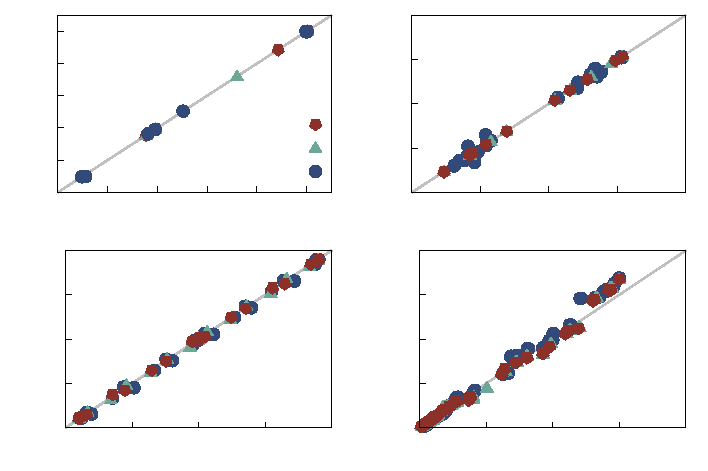
\includegraphics{mof-ff-validation}}%
    \gplfronttext
  \end{picture}%
\endgroup

    \caption{Comparisons of (a), (b) and (c): geometric parameters and (d):
    vibrational normal modes between the reference DFT data and the new MOF-FF
    force field.}
    \label{fig:fig:mof-ff:validation}
\end{figure}

We also extracted geometric parameters such as bonds lengths, or angles and
dihedral angles equilibrium value; as well as vibrational normal modes from the
same energy-minimized structures. We computed vibrational normal modes by using
finite differences to compute the full system Hessian in Cartesian coordinates;
and then diagonalizing the mass-weighted Hessian to extract normal modes
frequencies. These properties are compared to DFT calculations in
figure~\ref{fig:fig:mof-ff:validation}; and overall the new MOF-FF force field
is able to reproduce all of them very well. It overestimates the frequency of
vibrational modes after \SI{1500}{cm^{-1}}. These modes are very localized and
involve distortions of the linkers aromatic rings, which are not explicitly
described in the force field. A way to improve the description of these modes
would be to incorporate cross-terms (terms coupling multiples geometric
parameters, \ie a bond length and an angle, \dots) in the force field.

We then computed elastic constants of the frameworks with both DFT and MOF-FF,
the values are presented in table~\ref{tab:mof-ff:elastic}.
\citeauthor{Zheng2017} predicted recently the elastic constants of differently
functionalized ZIFs in the sod topology\cite{Zheng2017}. They found that
electron withdrawing groups improve the mechanical stiffness of the materials
(\ZIFCH3 < \ZIFCl < \ZIFBr). Although the absolute numbers of our DFT
calculations differ up to a few \si{GPa}, this trend is reproduced both by our
DFT and force field calculations.

\begin{figure}[hb]
    \centering
    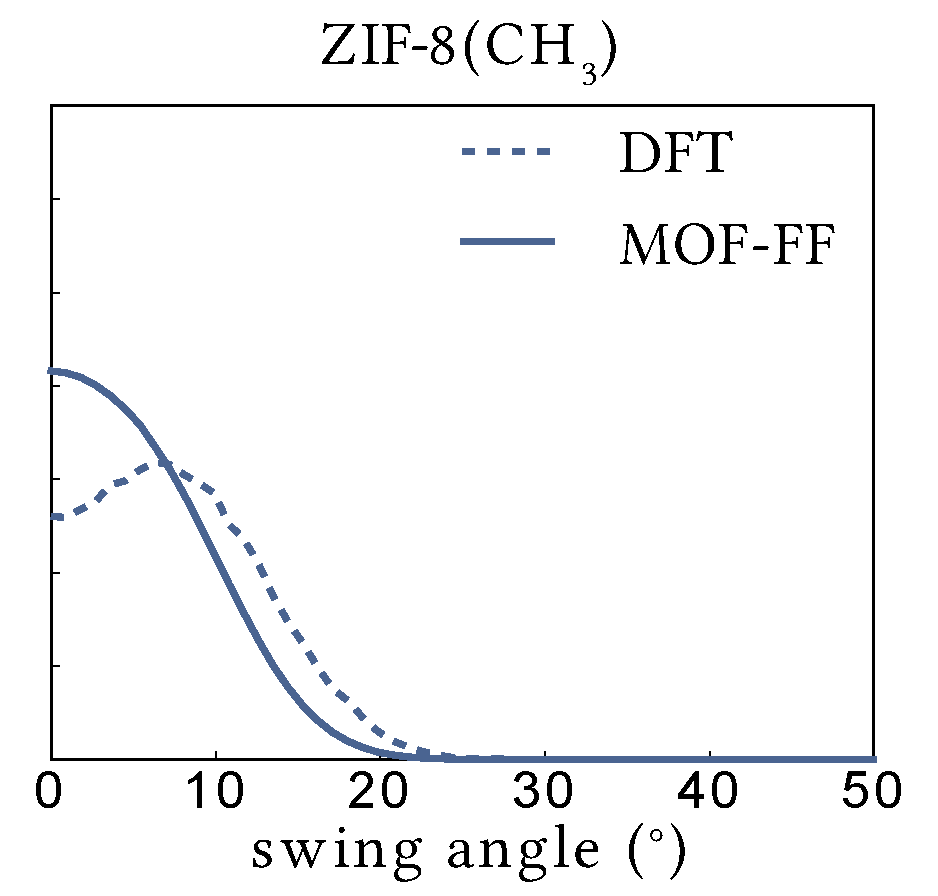
\includegraphics[width=0.32\textwidth]{figures/images/mof-ff-dihedrals-CH3}
    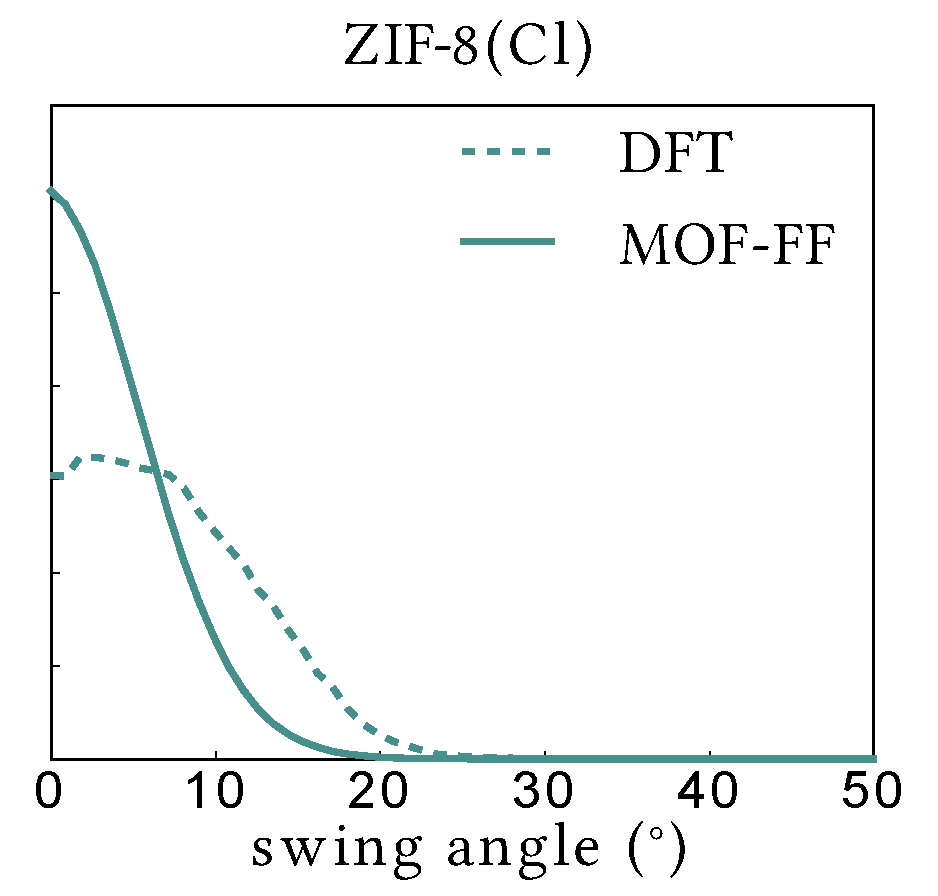
\includegraphics[width=0.32\textwidth]{figures/images/mof-ff-dihedrals-Cl}
    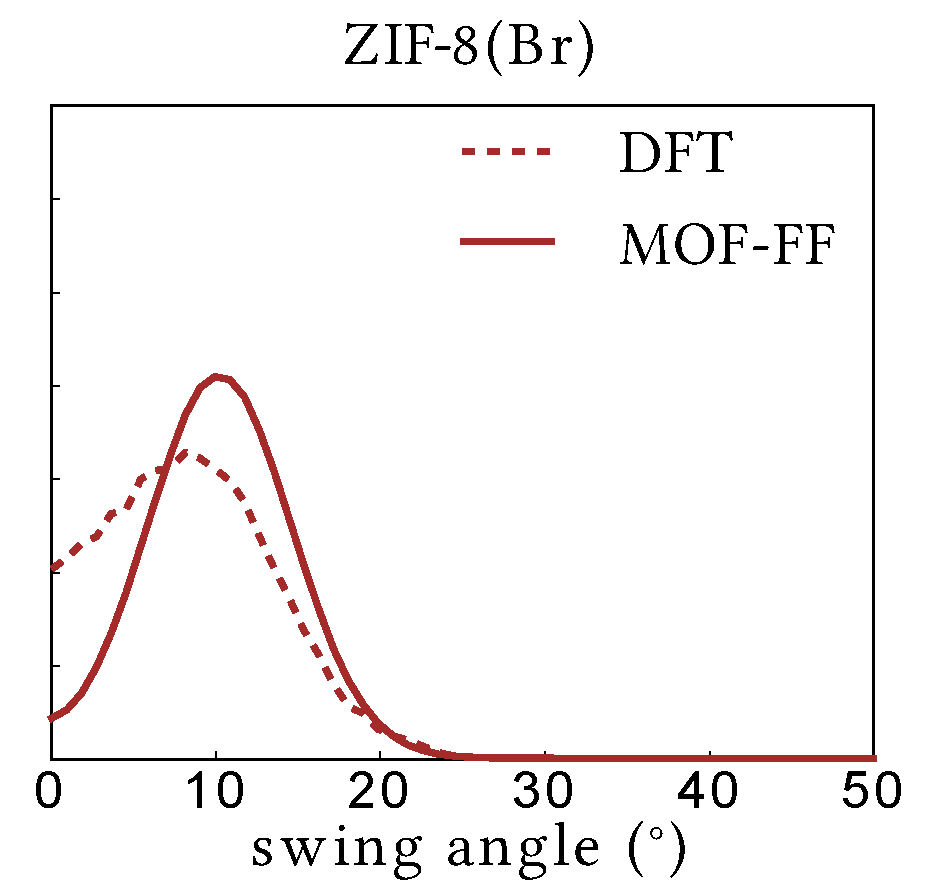
\includegraphics[width=0.32\textwidth]{figures/images/mof-ff-dihedrals-Br}
    \caption{Comparison of dihedral swing angle distribution in empty frameworks
    for the reference DFT simulations and the new MOF-FF force field.}
    \label{fig:fig:mof-ff:swing}
\end{figure}

Finally, we also ran constant temperature classical molecular dynamics using the
generated force field with the DL\_POLY software. From these simulations, we
computed the same swing angle distribution as in section~\ref{sec:zif8x:swing},
which are represented in figure~\ref{fig:fig:mof-ff:swing}. The general shape of
the DFT distributions is reproduced reasonably well by MOF-FF, but the central
value of the Gaussians is shifted by 5° for \ZIFCl and \ZIFBr; and by 10° for
\ZIFCH3. However, these differences are of the same order of magnitude as the
differences between the distributions generated by using a different DFT
functional such as BLYP\cite{Coudert2017}.

\FloatBarrier
\newpage
\section*{Conclusions}

First principles simulation methods are based on the Schrödinger equation.
Because solving this equation directly or numerically is difficult and limited
to very small systems, we use alternative methods such as DFT to find
approximated solutions. The main advantage of using such first principles
methods is that we don't need to make additional a priori approximations on the
shape of the energy surface.

I used DFT with molecular dynamics to study the adsorption of nitrogen in the
\ZIF8 MOF, and two other functionalized ZIF: \ZIFCl and \ZIFBr. I have shown
that in \ZIFCH3 and \ZIFCl, the linkers rotate around the plane of the 6 member
window when the nitrogen loading increases, creating a second step in the
adsorption isotherm. However, this linker rotation does not increase the
accessible porous volume in \ZIF8. Instead, it allows the nitrogen molecules to
re-organize inside the pore, from a packing to another. This repacking \emph{in
the same accessible volume} is at the origin of the second step in the nitrogen
adsorption isotherm. At the same time, the whole process of repacking and linker
rotation does not happen in \ZIFBr, probably because the pores are smaller in
\ZIFBr compared to \ZIFCH3 and \ZIFCl. This is also seen in the nitrogen
adsorption isotherm which does not present the second step.

I also used DFT calculations in collaboration with Johannes Dürholt and Rochus
Schmid to parametrize a classical force fields for the same structures.
Classical forces fields have the drawback of being less precise than \abinitio
calculations, and are usually not able to describe bonds creation and rupture.
They nonetheless have the advantage of being a lot cheaper to use to compute the
energy of large structures, allowing a better sampling of the phase space. In
the next chapter I will describe how I used classical simulations to study the
adsorption and intrusion of water and related fluids in hydrophobic porous
systems.

\OnlyInSubfile{\printglobalbibliography}

\end{document}
